% ============================================================
%  IEEE Conference Paper - IEEEtran class
%  Privacy-Preserving and Explainable Federated AI
%  for Alzheimer's & Dementia Detection
%  [REVISED - September 2026]
%
%  REVISION NOTE (read before compiling):
%  This revision restructures the paper so that the MNI-registered,
%  760-subject region study is the paper's subject, and the earlier
%  slice-space work appears only as (a) the leakage/orientation audit
%  that motivated the rebuild and (b) a clearly-scoped superseded arm.
%  Everything marked "% VERIFY:" needs a number or a fact the authors
%  hold and the editor does not.
%  Everything marked "% TODO-FIG:" needs a figure regenerated from the
%  v4 results; no v4 figure currently exists in figures/.
% ============================================================
\documentclass[10pt,conference]{IEEEtran}

% ---------- Core packages ----------
\usepackage[T1]{fontenc}
\usepackage[utf8]{inputenc}
\usepackage{cite}
\usepackage{amsmath}
\usepackage{amssymb}
\usepackage{amsfonts}
\usepackage{graphicx}
\usepackage{adjustbox}
\usepackage{textcomp}
\usepackage{xcolor}
\usepackage{booktabs}
\usepackage{multirow}
\usepackage{array}
\usepackage{url}
\usepackage{balance}
\usepackage[caption=false,font=footnotesize]{subfig}
\usepackage{tikz}
\usetikzlibrary{positioning,arrows.meta,shapes.geometric,fit,calc}

% ---------- Graphics path ----------
\graphicspath{{figures/}}

% ---------- Hyperref ----------
\usepackage[hidelinks,bookmarks=true,
  pdftitle={Privacy-Preserving and Explainable Federated AI
            for Alzheimer's and Dementia Detection}]{hyperref}

\interdisplaylinepenalty=2500
\setlength{\columnsep}{10pt}

% ============================================================
\begin{document}
% ============================================================

% Values below are written by src/paper_tables.py from results_summary.json.
% Do not edit by hand: run `python -m src.paper_tables` instead.
% BEGIN AUTO:facts
% --- Rebuilt (v3) cohort. Filled from results_v3/results_summary_v3.json. ---
\newcommand{\CohortAvailable}{2\,645}
\newcommand{\CohortADAvailable}{490}
\newcommand{\CohortTotal}{1\,002}
\newcommand{\CohortPerGroup}{334}
\newcommand{\CohortPerCell}{167}
\newcommand{\CohortAgeSpread}{0.7}
% --- Expanded (v4) cohort. Filled from results_v4/results_summary_v4.json. ---
\newcommand{\VFourBalN}{576}
\newcommand{\VFourBalTri}{50.8\%}
\newcommand{\VFourBalBin}{77.6\%}
% --- Confound analysis, from results_v4/metrics/confounds.json. Measured on
% --- the subjects for whom the demographic export supplies sex and age.
\newcommand{\ConfSexTri}{35.7\%}
\newcommand{\ConfAgeTri}{33.3\%}
\newcommand{\ConfImgTri}{51.2\%}
\newcommand{\ConfImgFemaleTri}{45.8\%}
\newcommand{\ConfImgMaleTri}{54.6\%}
\newcommand{\ConfNFemaleTri}{317}
\newcommand{\ConfNMaleTri}{321}
\newcommand{\ConfSexBin}{51.5\%}
\newcommand{\ConfImgBin}{80.1\%}
\newcommand{\ConfChanceTri}{34.0\%}
\newcommand{\ConfChanceBin}{50.6\%}
% --- The cohort this paper reports on, from results_v4/results_summary_v4.json.
\newcommand{\CohSubjects}{760}
\newcommand{\CohSites}{65}
\newcommand{\CohFeatures}{140}
\newcommand{\CohTriAcc}{52.5\%}
\newcommand{\CohTriF}{0.518}
\newcommand{\CohTriAUROC}{0.696}
\newcommand{\CohTriSite}{51.2\%}
\newcommand{\CohBinAcc}{78.9\%}
\newcommand{\CohBinSite}{77.4\%}
\newcommand{\CohBinAUROC}{0.862}
\newcommand{\CohDpBinOne}{71.6\%}
\newcommand{\CohDpBinTen}{78.4\%}
\newcommand{\CohDpBinNone}{75.1\%}
\newcommand{\CohXaiNonPrivate}{0.926}
\newcommand{\CohXaiTen}{0.437}
\newcommand{\CohMtNonPrivate}{12.9\%}
\newcommand{\CohMtTen}{12.4\%}
\newcommand{\CohDemog}{638}
% --- The initial, smaller cohort the study was first run on. Retained because
% --- the comparison between the two is itself a reported result.
\newcommand{\InitSubjects}{297}
\newcommand{\InitSites}{42}
\newcommand{\InitTriAcc}{51.1\%}
\newcommand{\InitBinAcc}{79.7\%}
\newcommand{\InitXaiTen}{0.062}
\newcommand{\InitSexOnly}{41.4\%}
\newcommand{\ChanceAccuracy}{33.3\%}
\newcommand{\BestNonPrivateAcc}{36.1\%}
% END AUTO:facts

% Convenience macros for the superseded slice-space arm, so that a reader
% never has to guess which cohort a number belongs to.
\newcommand{\slicearm}{superseded slice pipeline}
\newcommand{\AuditSubjects}{32}
\newcommand{\SliceSubjects}{299}

\title{Privacy-Preserving and Explainable Federated AI\\
       for Alzheimer's \& Dementia Detection}

\author{%
  \IEEEauthorblockN{%
    Adit Srivastava\IEEEauthorrefmark{1},\;
    Aditya Raj\IEEEauthorrefmark{2},\;
    Vaibhav Gupta\IEEEauthorrefmark{3},\;
    Hardik Gupta\IEEEauthorrefmark{4},\;
    Agha Alfi Mirza\IEEEauthorrefmark{5}%
  }\\[4pt]
  \IEEEauthorblockA{%
    \IEEEauthorrefmark{1}\IEEEauthorrefmark{2}%
    \IEEEauthorrefmark{3}%
    Department of Computer Science \& Engineering,
    PES University, Bangalore, India\\
    \IEEEauthorrefmark{4}%
    Department of Electronics \& Communication Engineering,
    PES University, Bangalore, India\\
    \IEEEauthorrefmark{5}%
    Project Guide, Department of Computer Science \& Engineering,
    PES University, Bangalore, India\\[2pt]
    \{PES1UG23AM017, PES1UG23CS034, PES1UG23AM341,
       PES1UG23EC115\}@pes.edu
  }%
}

\maketitle

% ============================================================
\begin{abstract}
Deep learning on MRI is a promising route to earlier Alzheimer's disease
detection, but privacy regulation blocks the cross-institutional pooling such
models are usually trained on.  This paper reports a privacy-preserving and
explainable federated study on \CohSubjects{}~ADNI subjects across
\CohSites{}~sites, and is as much about how such systems are measured as about
the systems themselves.  We document and correct two measurement defects in our
own earlier pipeline.  The first, slice-level splitting, let scans of the same
patient reach both training and test data and inflated federated accuracy to
97.0\%.  The second, reported here, explains the residual: the pipeline chose
its slice axis as the longest array axis, which extracts a sagittal plane for
some subjects, an axial plane for others and a coronal plane for the rest,
decided by how the scanner wrote the file.  It raises no error.  Compounding
it, 272 of the 620 scans in the initial download carry a degenerate identity
affine from which orientation cannot be read.  We recover orientation by
registration search over all 48~axis permutations and reflections against a
whole-head template, anchored on four subjects holding both a degenerate scan
and one with a usable header.

With every subject registered to MNI152 and represented by
\CohFeatures{}~grey-matter and CSF fractions over Harvard-Oxford regions,
three-class accuracy reaches \CohTriAcc{} (macro F1~\CohTriF{},
AUROC~\CohTriAUROC{}) and CN versus AD reaches \CohBinAcc{}
(AUROC~\CohBinAUROC{}) under a subject-disjoint protocol, with a model four
orders of magnitude smaller than the network it replaces; a site-disjoint
evaluation gives \CohTriSite{} and \CohBinSite{}.  We federate over the
\CohSites{}~real ADNI sites rather than a simulated partition.  Subject-level
differential privacy over the region model stays usable down to
$\varepsilon = 1$ (\CohDpBinOne{} on CN versus AD) where the full network
collapses onto the majority class; we attribute this to the perturbed dimension
via the standard $\sigma C\sqrt{d}$ scaling of the Gaussian mechanism, measured
here on one mechanism and one cohort at $d = 423$, $d = 6{,}147$ and
$d = 2.35\times10^{7}$.  Finally, because every feature is a named anatomical
region, attributions are comparable across models: agreement with the
non-private reference falls from \CohXaiNonPrivate{} to \CohXaiTen{} at
$\varepsilon = 10$, a budget at which accuracy does not fall, so accuracy-only
privacy--utility curves understate what a private model costs wherever the
explanation is part of the deliverable.  We release the corrected pipeline, the
measured orientation table, the subject-level and site-level splits, and all
runs.
\end{abstract}

\begin{IEEEkeywords}
Federated Learning, Alzheimer's Disease, Differential Privacy,
Explainable AI, Evaluation Methodology, Data Leakage, MRI
Registration, Region-Based Morphometry, ADNI, HIPAA, GDPR
\end{IEEEkeywords}

% ============================================================
\section{Introduction}
\label{sec:intro}
% ============================================================

Alzheimer's Disease~(AD) is the most prevalent cause of dementia
worldwide, affecting over 55~million individuals---a figure projected
to exceed 150~million by 2050~\cite{pan2025}.  The disease is
characterised by progressive neurodegeneration involving hippocampal
atrophy, cortical thinning, and ventricular enlargement, which are
detectable through structural Magnetic Resonance Imaging~(MRI) well
before clinical symptom onset~\cite{adni}.  Early and accurate diagnosis
at the mild cognitive impairment~(MCI) stage is therefore critical, as
timely interventions can significantly slow disease progression and
improve patient quality of life.

Deep learning has transformed medical image analysis, and convolutional
architectures such as VGG19~\cite{vgg19} and ResNet50~\cite{resnet50}
report strong numbers on neuroimaging benchmarks when trained on large
centralised datasets.  Deployment across institutions, however, faces a
hard barrier: patient data privacy.  HIPAA in the United States and
GDPR in the European Union restrict cross-institutional sharing of
protected health information, so training a single generalisable model
over pooled hospital data is legally infeasible.

Federated Learning~(FL)~\cite{mcmahan2017} answers this by keeping data
local and communicating only model updates, aggregated on a server by
Federated Averaging (FedAvg).  FL for Alzheimer's detection has been
demonstrated by Mitrovska et al.~\cite{mitrovska2024} and by Pan et
al.~\cite{pan2025}.  Standard FL is nonetheless vulnerable to
gradient-inversion~\cite{zhu2019} and membership-inference attacks, and
Differential Privacy~(DP)~\cite{dwork2014,abadi2016} bounds that leakage
at a cost in utility.  Separately, clinical deployment demands
transparency, which Explainable AI~(XAI) methods such as
Grad-CAM~\cite{gradcam} and SHAP~\cite{shap} are intended to supply.

This paper is a corrected re-report of our own system, and its
contributions are as much about measurement as about method.  An
earlier version of this work reported 91--97\% accuracy from a
pipeline containing two defects, either of which alone would have
invalidated the headline.  Both are documented here, and the pipeline
was rebuilt around their causes.  Our contributions are:

\begin{enumerate}
\item \textbf{Two measurement defects, quantified.}\;We show on
      identical data and architectures that slice-level rather than
      subject-level splitting inflated held-out accuracy from
      19--36\% to 91--97\%.  We then show that the residual
      chance-level accuracy was not, as we previously argued, a
      consequence of cohort size: the pipeline selected its slice axis
      as the longest array axis, which extracts a different anatomical
      plane depending only on how each scanner wrote the file
      (Section~\ref{sec:standardisation}).  The second defect raises no
      error and is invisible to any downstream metric.

\item \textbf{A measured orientation table for degenerate-affine ADNI
      series.}\;272 of the 620 scans in the initial download carry an
      identity affine from which orientation cannot be read.  We
      recover it by registration search over all 48~axis permutations
      and reflections against a whole-head template, resolve the
      left--right mirror on four within-subject anchors, and release
      the resulting per-series table
      (Table~\ref{tab:orientation-table}).

\item \textbf{A standardised region representation and its
      evaluation.}\;With every subject on the MNI152 grid and described
      by \CohFeatures{}~grey-matter and CSF fractions over
      Harvard-Oxford regions, a \mbox{423-parameter} model reaches
      \CohTriAcc{} on three classes and \CohBinAcc{} on CN versus AD,
      reported under both subject-disjoint and site-disjoint protocols
      (Section~\ref{sec:results-centralised}).

\item \textbf{Federation over the real ADNI site partition}, compared
      against IID and Dirichlet partitions of the same subjects, so
      that the effect of using the cohort's own heterogeneity is
      measured rather than asserted
      (Section~\ref{sec:results-federated}).

\item \textbf{Subject-level DP-FedAvg and a dimensional account of its
      cost.}\;The usable regime of the Gaussian mechanism is fixed by
      the perturbed dimension, a point established in the DP
      literature~\cite{bassily2014,tramer2021} that we measure here on
      one mechanism and one clinical cohort across
      $d = 423$, $6{,}147$ and $2.35\times10^{7}$
      (Section~\ref{sec:dimension-law}).

\item \textbf{An explanation-fidelity analysis that a slice pipeline
      cannot support.}\;Because features are named regions,
      attributions are comparable across models rather than merely
      displayable, and we report both a model-anchored and an
      anatomy-anchored measure of how DP moves them
      (Section~\ref{sec:results-xai}).

\item \textbf{A demographic-confound analysis and a balanced cohort
      specification}, so that an imaging claim is separated from what
      sex and age alone could produce
      (Sections~\ref{sec:results-confounds}--\ref{sec:cohort-design}).
\end{enumerate}

Section~\ref{sec:related} reviews related work.
Section~\ref{sec:problem} formalises the problem.
Section~\ref{sec:architecture} presents the system.
Section~\ref{sec:methodology} details the methodology, including both
defects and their corrections.
Sections~\ref{sec:setup} and~\ref{sec:results} cover experimental setup
and results, with the superseded slice-space arm confined to
Section~\ref{sec:legacy}.
Section~\ref{sec:privacy} analyses privacy,
Section~\ref{sec:verification} reproducibility, and
Sections~\ref{sec:limitations}--\ref{sec:conclusion} limitations, future
work and conclusions.

% ============================================================
\section{Related Work}
\label{sec:related}
% ============================================================

\subsection{Alzheimer's Detection from Structural MRI}

Two families of method dominate.  The first summarises anatomy into
region or voxel features and classifies them with a linear or kernel
model.  Kl\"{o}ppel et al.~\cite{kloppel2008} established the approach
on whole-brain grey matter, and Cuingnet et al.~\cite{cuingnet2011}
compared ten such methods on a common ADNI cohort under a fixed
protocol, which remains the reference point for what a well-built
morphometric baseline achieves: CN versus AD in the low-to-mid eighties,
CN versus MCI substantially lower.
% VERIFY: replace the qualitative range above with the exact figures you
% wish to quote from Cuingnet et al., Table 3, before submission.
The second family trains CNNs (VGG~\cite{vgg19}, ResNet~\cite{resnet50},
AlexNet) end-to-end on slices or volumes; an evolutionary FL
approach~\cite{evolutionary2025} reports 98.53\% on ADNI with
genetic-algorithm hyperparameter search over a multimodal input.

We position our region representation against the first family
deliberately.  It is not a new representation, and we do not claim it
as one: it is a forty-year-old idea whose value here is that it is
low-dimensional, anatomically named, and therefore both cheap under DP
and comparable across models.  Section~\ref{sec:results-centralised}
reports our numbers against that literature rather than only against our
own earlier pipeline.

\subsection{Federated Learning in Healthcare}

McMahan et al.~\cite{mcmahan2017} proposed FedAvg.  Mitrovska et
al.~\cite{mitrovska2024} applied secure FL to AD detection on ADNI MRI,
reporting 94\% accuracy with secure aggregation~\cite{bonawitz2017}.
Pan et al.~\cite{pan2025} deployed FL across six real healthcare sites
for MCI-to-AD progression, reporting 85\% AUROC.  Kairouz et
al.~\cite{kairouz2021} survey the open problems, of which non-IID
heterogeneity is the one most often simulated and least often measured
on a real partition.  Most ADNI FL work draws client partitions from a
Dirichlet distribution; we report that draw alongside the cohort's own
site partition (Section~\ref{sec:results-federated}).

\subsection{Differential Privacy, and the Role of Dimension}
\label{sec:related-dp}

DP~\cite{dwork2014} bounds leakage from released updates, and
DP-SGD~\cite{abadi2016} is the standard mechanism.  McMahan et
al.~\cite{mcmahan2018} give the federated, user-level variant we adopt,
in which the unit of privacy is a whole participant rather than a single
training example.  Kaissis et al.~\cite{privacy2024} integrate DP with
uncertainty quantification for federated medical imaging.

The dependence of DP utility on the perturbed dimension is established.
Bassily et al.~\cite{bassily2014} give the dimension-dependent error
bounds for private empirical risk minimisation; Tram\`{e}r and
Boneh~\cite{tramer2021} argue directly that private learning on modest
data is better served by good low-dimensional features than by
end-to-end deep networks, and demonstrate handcrafted features beating
CNNs under DP; Yu et al.~\cite{yu2021} attack the same problem by
projecting gradients into a low-dimensional subspace.
Section~\ref{sec:dimension-law} does not claim this insight.  What it
contributes is a measurement of the resulting regime on a single
mechanism and a single clinical cohort at three dimensionalities
spanning five orders of magnitude, together with the failure mode
(majority-class collapse) that the high-dimensional end produces and
that an accuracy-only curve reports as a success.

\subsection{Explainable AI in Medical Imaging}

Selvaraju et al.~\cite{gradcam} proposed Grad-CAM and Lundberg and
Lee~\cite{shap} SHAP.  Mastoi et al.~\cite{mastoi2025} combine FL with
both for brain tumour classification.  Pan et al.~\cite{pan2025} apply
SHAP in a federated clinical-variable setting.  A property common to the
imaging work is that explanations are displayed rather than compared:
without registration, a heat map at pixel~$(i,j)$ refers to different
anatomy in different subjects, so it can be shown to a reader but not
averaged over subjects or correlated between models.  Registration to a
common template and attribution over named regions removes that
obstacle, which is what makes the analysis of
Section~\ref{sec:results-xai} possible at all.

\subsection{Evaluation Practice in Small Neuroimaging Cohorts}

Subject-level leakage in slice-classification pipelines is a known
hazard and an under-reported one.  We are not aware of a published ADNI
slice-classification result that explicitly confirms subject-disjoint
splitting, and we make no claim about any specific prior work; our own
earlier pipeline is the only one we can audit directly, and
Section~\ref{sec:leakage} audits it.

\subsection{Summary and Research Gap}

Table~\ref{tab:lit_review} summarises the reviewed work.  The gap this
paper addresses is narrower and, we think, more defensible than the
four-way feature checklist an earlier version of this paper claimed.
Privacy, accuracy and explainability have all been combined before in
some pairing.  What has not been reported, on Alzheimer's MRI, is a
pipeline in which (i)~the anatomical plane every subject contributes is
measured rather than assumed, (ii)~the privacy unit is the patient
rather than the slice, (iii)~the federated partition is the cohort's own
sites rather than a simulated draw, and (iv)~the explanation is defined
over named regions and is therefore comparable between a private model
and its non-private reference.

\begin{table*}[t]
  \centering
  \caption{Summary of Related Work}
  \label{tab:lit_review}
  \renewcommand{\arraystretch}{1.15}
  \setlength{\tabcolsep}{3.5pt}
  \footnotesize
  \begin{tabular}{p{3.0cm}lp{2.6cm}lp{2.2cm}p{3.2cm}}
    \toprule
    \textbf{Authors} & \textbf{Domain} &
    \textbf{Method} & \textbf{Dataset} &
    \textbf{Key Result} & \textbf{Limitation / Gap} \\
    \midrule
    Cuingnet et al.~\cite{cuingnet2011}
      & Morphometry
      & 10 methods, fixed protocol
      & ADNI (509 subj.)
      & Reference baselines
      & Centralised; no privacy or XAI \\
    \addlinespace
    Mitrovska et al.~\cite{mitrovska2024}
      & FL + Privacy
      & FedAvg + SecAgg
      & ADNI
      & 94\% Acc.
      & No XAI; limited DP analysis \\
    \addlinespace
    Mastoi et al.~\cite{mastoi2025}
      & FL + XAI
      & FL + Grad-CAM + SHAP
      & Brain tumour
      & $>$90\% Acc.
      & Not AD-specific; no DP; pixel-space XAI \\
    \addlinespace
    Pan et al.~\cite{pan2025}
      & FL + Clinical
      & FL + SHAP (EHR)
      & Multi-site EHR
      & 85\% AUROC
      & EHR-based; no MRI; no DP \\
    \addlinespace
    Kaissis et al.~\cite{privacy2024}
      & DP + Medical
      & FL + DP + Uncertainty
      & Medical imaging
      & 92--95\% retained
      & Not AD-specific; no XAI \\
    \addlinespace
    Tram\`{e}r \& Boneh~\cite{tramer2021}
      & DP + Features
      & Handcrafted features under DP
      & CIFAR/MNIST
      & Features beat CNNs under DP
      & Not medical; no FL \\
    \addlinespace
    McMahan et al.~\cite{mcmahan2018}
      & User-level DP
      & DP-FedAvg
      & Language
      & User-level $(\varepsilon,\delta)$
      & Not medical; no XAI \\
    \midrule
    \textbf{PPXFL (Ours)}
      & \textbf{FL+DP+XAI}
      & \textbf{Measured orientation; MNI region features; DP-FedAvg; region attribution}
      & \textbf{ADNI MRI (\CohSubjects{}~subj., \CohSites{}~sites)}
      & \textbf{\CohBinAcc{} CN/AD; usable to $\varepsilon{=}1$; attribution agreement \CohXaiNonPrivate{}$\to$\CohXaiTen{}}
      & \textbf{No MIA on the region model (Sec.~\ref{sec:limitations})} \\
    \bottomrule
  \end{tabular}
\end{table*}

% ============================================================
\section{Problem Statement}
\label{sec:problem}
% ============================================================

\subsection{The Real-World Challenge}

Diagnosis of AD from structural MRI relies on manual radiological
assessment---subjective and subject to inter-rater
variability~\cite{adni}---or on centralised models that require pooled
data.  In practice scans reside across geographically distributed
hospitals under distinct review boards.  Sharing raw MRI across
institutions is restricted by HIPAA, GDPR and analogous regulation, so
each hospital trains on its own limited data, with small samples,
demographic bias and poor generalisation.

\subsection{Why Existing Approaches Are Insufficient}

Centralised deep learning~\cite{vgg19,resnet50} violates data
sovereignty.  Standard FL~\cite{mcmahan2017} keeps data local but
remains vulnerable to gradient inversion~\cite{zhu2019} and membership
inference.  Prior privacy-protected FL
systems~\cite{mitrovska2024,privacy2024} do not provide explanations in
a form that can be compared across models.  And, as this paper's own
history shows, a pipeline can satisfy every architectural requirement
above while producing a number that means nothing, because the defect
lies in how the data was cut and how each volume was indexed rather than
in the learning at all.

\subsection{Formal Problem Definition}

Let $\mathcal{C}=\{C_1,\ldots,C_K\}$ denote $K$ hospital clients, each
holding a local dataset
$\mathcal{D}_k=\{(x_i^{(k)},y_i^{(k)})\}_{i=1}^{n_k}$, where
$x_i^{(k)}\in\mathcal{X}$ is a subject's representation --- in this
paper, either a vector of $\CohFeatures{}$ region fractions computed on
the MNI152 grid or a stack of registered slices at named MNI
coordinates --- and $y_i^{(k)}\in\{0,1,2\}$ is the diagnostic label
(0=CN, 1=MCI, 2=AD).  Each subject appears in exactly one client.

The objective is to learn a global classifier
$f_{\theta}:\mathcal{X}\rightarrow[0,1]^3$ minimising the weighted
population risk
\begin{equation}
  \min_{\theta}\;\mathcal{L}(\theta)
  = \sum_{k=1}^{K}\frac{n_k}{n}\,\mathcal{L}_k(\theta),
  \label{eq:global_obj}
\end{equation}
with $n=\sum_k n_k$, subject to two constraints:
\begin{enumerate}
\item \textbf{Data locality:} no raw data $x_i^{(k)}$ leaves client
  $C_k$; only updates $\Delta\theta^{(k)}$ are communicated.
\item \textbf{Subject-level privacy:} the released model must satisfy
  $(\varepsilon,\delta)$-DP with respect to the inclusion or exclusion
  of \emph{an entire subject}, not a single slice.  This is the
  guarantee a hospital needs and the weaker slice-level unit does not
  provide, since a patient contributes many slices.
\end{enumerate}

\subsection{A Third Constraint the Formalism Hides}

Equation~\eqref{eq:global_obj} presumes that $x_i^{(k)}$ means the same
thing for every $i$ and every $k$.  On raw ADNI it does not.  Volumes
arrive in native scanner space at voxel sizes from $0.94$ to
$1.25$~mm, unregistered and unstripped, in several stored array orders,
and a substantial fraction carry affines from which orientation cannot
be read at all.  A pipeline that indexes those volumes by array
position, as ours did, silently feeds different anatomy to the same
input coordinate for different subjects.  No loss function, privacy
accountant or explanation method detects this.  Anatomical
standardisation is therefore not preprocessing hygiene here; it is a
precondition for the problem statement to be well posed, and
Section~\ref{sec:standardisation} treats it as one.

% ============================================================
\section{System Architecture}
\label{sec:architecture}
% ============================================================

The architecture is shown in Fig.~\ref{fig:architecture} and comprises
five stages.

\textbf{Standardisation Stage (local, once).}\;Each site orients its own
volumes using the measured per-series table
(Table~\ref{tab:orientation-table}), skull-strips with deepbet, and
registers to MNI152 2~mm.  Region fractions are then computed locally.
This stage runs inside the client boundary and produces the
representation everything downstream consumes; no raw or registered
volume leaves the site.

\textbf{Client Layer (real ADNI sites).}\;One client per site, with
sites below a minimum size pooled so that no subject is discarded.
Each client trains a local copy of the global model on its own subjects
and returns a parameter delta.  IID and Dirichlet partitions of the same
subjects are also evaluated, as controls against which the real
partition is compared.

\textbf{Federated Server.}\;Orchestrates $T$ rounds: samples $q|S|$
subjects, receives clipped deltas, aggregates by FedAvg
(Eq.~\eqref{eq:fedavg}), and applies the subject-level Gaussian
mechanism (Section~\ref{sec:dp-mechanism}) before redistributing.

\textbf{Privacy Module (subject-level DP).}\;Each subject's total
contribution is clipped to $C$ in $L_2$ before noise, so the released
model satisfies $(\varepsilon,\delta)$-DP with the subject as the unit.
The perturbed dimension is a design parameter, not a fixed property of
the mechanism, and Section~\ref{sec:dimension-law} shows it is the
parameter that decides usability.

\textbf{Explainability and Evaluation.}\;Attribution is computed per
named Harvard-Oxford region, which makes two models' explanations
directly comparable and makes an anatomy-anchored check
(share of attribution mass in hippocampus and amygdala) meaningful.
Evaluation reports utility under both subject-disjoint and
site-disjoint splits, the demographic-confound baselines, and the
attribution measures.

% --- TikZ Architecture Diagram (rewritten for the actual system) ---
\begin{figure*}[t]
  \centering
  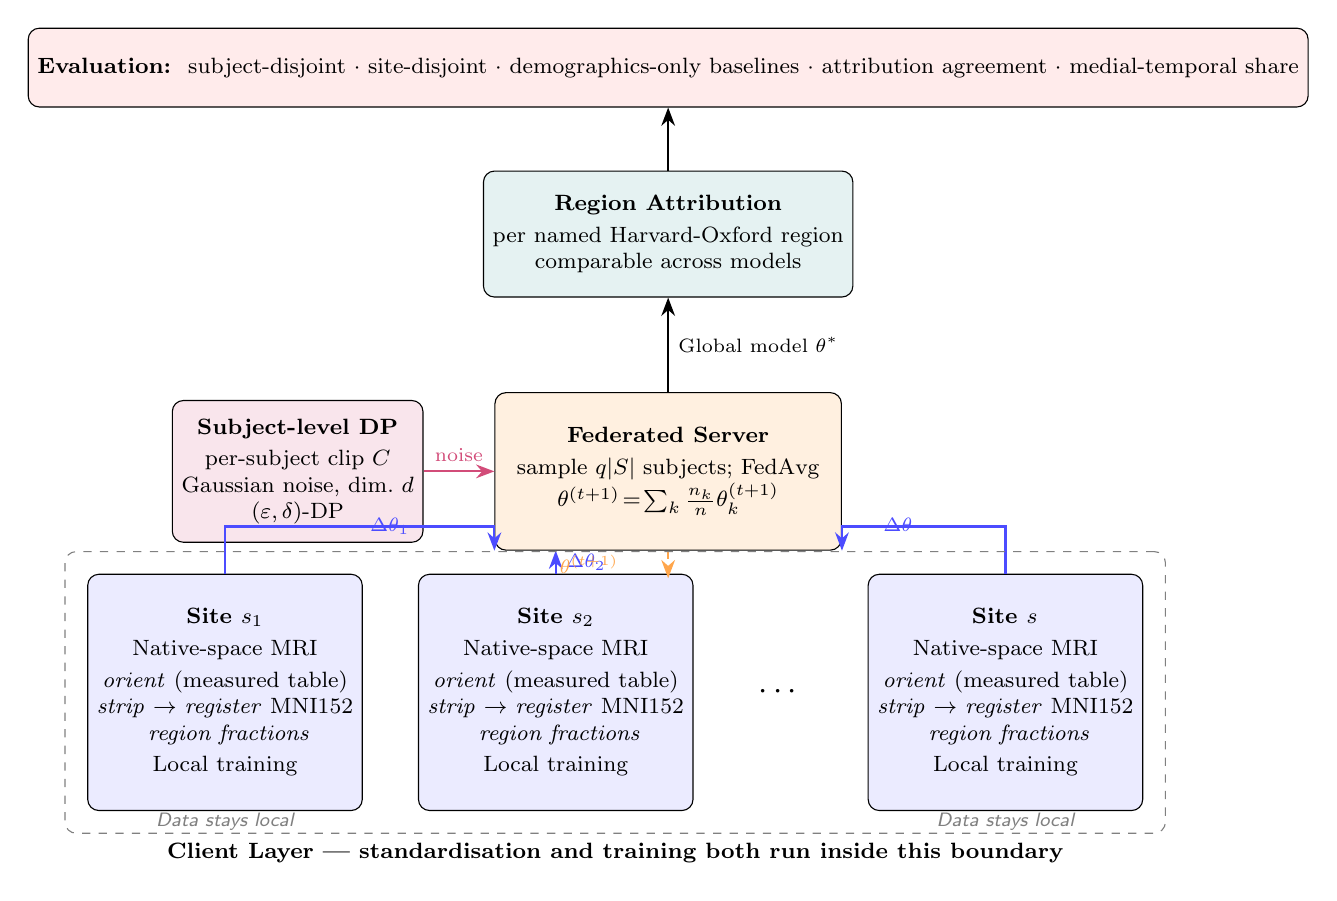
\begin{tikzpicture}[
    >=Stealth,
    node distance=1.0cm and 1.2cm,
    clientbox/.style={draw, rounded corners, fill=blue!8,
      minimum width=3.0cm, minimum height=3.0cm, align=center,
      font=\footnotesize},
    serverbox/.style={draw, rounded corners, fill=orange!12,
      minimum width=4.4cm, minimum height=2.0cm, align=center,
      font=\footnotesize},
    modulebox/.style={draw, rounded corners, fill=green!8,
      minimum width=3.0cm, minimum height=1.6cm, align=center,
      font=\footnotesize},
    evalbox/.style={draw, rounded corners, fill=red!8,
      minimum width=11cm, minimum height=1.0cm, align=center,
      font=\footnotesize},
    arrowstyle/.style={->, thick, >=Stealth},
    dashedarrow/.style={->, thick, dashed, >=Stealth},
    lbl/.style={font=\scriptsize\itshape, text=gray}
  ]
    % --- Client nodes ---
    \node[clientbox] (c1) {%
      \textbf{Site $s_1$}\\[2pt]
      Native-space MRI\\[2pt]
      \textit{orient} (measured table)\\
      \textit{strip} $\rightarrow$ \textit{register} MNI152\\
      \textit{\CohFeatures{} region fractions}\\[2pt]
      Local training};
    \node[clientbox, right=0.7cm of c1] (c2) {%
      \textbf{Site $s_2$}\\[2pt]
      Native-space MRI\\[2pt]
      \textit{orient} (measured table)\\
      \textit{strip} $\rightarrow$ \textit{register} MNI152\\
      \textit{\CohFeatures{} region fractions}\\[2pt]
      Local training};
    \node[font=\large, right=0.7cm of c2] (dots) {$\cdots$};
    \node[clientbox, right=0.7cm of dots] (cK) {%
      \textbf{Site $s_{\CohSites{}}$}\\[2pt]
      Native-space MRI\\[2pt]
      \textit{orient} (measured table)\\
      \textit{strip} $\rightarrow$ \textit{register} MNI152\\
      \textit{\CohFeatures{} region fractions}\\[2pt]
      Local training};

    \node[lbl, below=-0.1cm of c1] {\textsf{Data stays local}};
    \node[lbl, below=-0.1cm of cK] {\textsf{Data stays local}};

    % --- Federated Server ---
    \node[serverbox, above=1.8cm of $(c2)!0.5!(dots)$] (server) {%
      \textbf{Federated Server}\\[2pt]
      sample $q|S|$ subjects; FedAvg\\
      $\theta^{(t+1)}\!=\!\sum_k\frac{n_k}{n}\theta_k^{(t+1)}$};

    % --- DP Module ---
    \node[modulebox, fill=purple!10, left=0.9cm of server,
      minimum width=2.6cm, minimum height=1.8cm] (dp) {%
      \textbf{Subject-level DP}\\[2pt]
      per-subject clip $C$\\
      Gaussian noise, dim.\ $d$\\
      $(\varepsilon,\delta)$-DP};

    \draw[arrowstyle, blue!70] (c1.north) -- ++(0,0.6) -| (server.south west)
      node[pos=0.25, right, font=\scriptsize] {$\Delta\theta_1$};
    \draw[arrowstyle, blue!70] (c2.north) -- (server.south -| c2)
      node[pos=0.5, right, font=\scriptsize] {$\Delta\theta_2$};
    \draw[arrowstyle, blue!70] (cK.north) -- ++(0,0.6) -| (server.south east)
      node[pos=0.25, left, font=\scriptsize] {$\Delta\theta_{\CohSites{}}$};

    \draw[arrowstyle, purple!70] (dp.east) -- (server.west)
      node[midway, above, font=\scriptsize] {noise};

    % --- XAI Layer ---
    \node[modulebox, fill=teal!10, above=1.2cm of server] (xai) {%
      \textbf{Region Attribution}\\[2pt]
      per named Harvard-Oxford region\\
      comparable across models};

    \draw[arrowstyle] (server.north) -- (xai.south)
      node[midway, right, font=\scriptsize] {Global model $\theta^*$};

    \node[evalbox, above=0.8cm of xai] (eval) {%
      \textbf{Evaluation:}\;
      subject-disjoint $\cdot$ site-disjoint $\cdot$
      demographics-only baselines $\cdot$
      attribution agreement $\cdot$ medial-temporal share};

    \draw[arrowstyle] (xai.north) -- (eval.south);

    \draw[dashedarrow, orange!70] (server.south) -- ++(0,-0.35)
      node[midway, left, font=\scriptsize, xshift=-5mm] {$\theta^{(t+1)}$};

    \node[draw, dashed, gray, rounded corners, inner sep=8pt,
      fit=(c1)(c2)(dots)(cK), label={[font=\footnotesize\bfseries]below:%
      Client Layer --- standardisation and training both run inside this boundary}] {};

  \end{tikzpicture}
  \caption{System architecture.  Anatomical standardisation
    (orientation from the measured per-series table, skull stripping,
    MNI152 registration, region-fraction extraction) runs \emph{inside}
    the client boundary, so the representation that leaves a site is
    already a model update over named regions.  Clients are the
    \CohSites{}~real ADNI sites; IID and Dirichlet partitions of the
    same subjects are evaluated as controls.  The server applies the
    subject-level Gaussian mechanism, whose perturbed dimension~$d$ is
    the design parameter that
    Section~\ref{sec:dimension-law} identifies as decisive.  No raw or
    registered volume crosses the dashed boundary.}
  \label{fig:architecture}
\end{figure*}

% ============================================================
\section{Methodology}
\label{sec:methodology}
% ============================================================

\subsection{Anatomical Standardisation}
\label{sec:standardisation}

The pipeline used in the previous version of this study selected its slice
axis as the longest array axis,
\texttt{axial\_axis = np.argmax(data.shape)}, and took three slices around the
midpoint of that axis. Over the cohort actually downloaded, that rule does not
select a consistent anatomical plane. Table~\ref{tab:orientation-defect} lists
what it extracts for the three stored layouts present in the data: a sagittal
plane for volumes written as $(256, 240, 160)$ in RAS order, an axial plane for
volumes written as $(256, 256, 166)$ in IPL order, and a coronal plane for
volumes written as $(166, 256, 256)$. The plane a subject contributes is
therefore decided by how its scanner wrote the file rather than by anatomy, and
no downstream stage can recover from it. Three further properties of the raw
download compound the problem: the volumes are in native scanner space with
voxel sizes from $0.94$ to $1.25$~mm and are never registered, so no voxel
index corresponds between subjects; they are not skull-stripped, so skull, face
and neck remain in frame; and the download contains up to five ADNI
preprocessing levels of the same acquisition, which the file glob treated as
independent samples.

\begin{table}[t]
\centering
\caption{What the previous slice rule extracts, by stored layout.}
\label{tab:orientation-defect}
\begin{tabular}{lllc}
\toprule
Stored shape & Orientation & Axis chosen & Plane extracted \\
\midrule
$(256, 240, 160)$ & RAS & 0 & sagittal \\
$(256, 256, 166)$ & IPL & 0 & axial \\
$(166, 256, 256)$ & RAS & 1 & coronal \\
\bottomrule
\end{tabular}
\end{table}

The rebuilt pipeline places every subject in a common anatomical space. One
scan is retained per subject, chosen by preprocessing level and then by
earliest visit, with the derived \texttt{Mask} and \texttt{HarP} products
excluded because they are binary label volumes rather than intensity images.
Each scan is then oriented, skull-stripped with deepbet, and registered to the
MNI152 2~mm template by mutual information over a translation, rigid and
affine sequence. A per-subject quality score, the Pearson correlation with the
template inside the brain mask, is recorded so that failures are excluded by a
stated rule rather than by inspection.

\subsubsection{Recovering orientation from scans without a usable affine}
\label{sec:orientation}

Orientation cannot simply be read from the header. Of the 620 usable scans in
the initial download, 272 --- the raw \texttt{MPRAGE} and
\texttt{Accelerated\_SAG\_IR-SPGR} series --- carry an identity affine with
\texttt{sform\_code}~$=2$ and \texttt{qform\_code}~$=0$. For those files
\texttt{nibabel.as\_closest\_canonical} reports RAS and leaves the array order
untouched, even though the acquisition is sagittal and the stored order is not
RAS at all. This is the reason the slice defect above was not visible as an
error.
% VERIFY: state here, in one sentence, the relationship between the 620-scan
% initial download and the 760-subject cohort of Section VI-A -- specifically
% whether the expanded download introduced any series group not present in
% Table III, and if so what was done. A reader will otherwise read "620 usable
% scans" and "760 subjects" as a contradiction.
The orientation table below was fitted on the initial download and applied
unchanged to the expanded cohort; every series group present in the expansion
appears in Table~\ref{tab:orientation-table}.

The orientation is therefore measured rather than assumed. For each of the 48
axis permutations and reflections, the candidate volume is registered to a
4~mm whole-head ICBM152 target and scored by correlation. Two design points
matter. First, the target must retain the skull: the scan being oriented has
not been stripped yet, and matching an unstripped head against a
skull-stripped brain scored $0.09$--$0.48$ and selected a different, incorrect
orientation on the same subjects, where head-to-head matching scores
$0.68$--$0.79$ for the correct candidate with a clear margin to the third. This
also forces the ordering of the pipeline: deepbet is trained on anatomically
oriented volumes and leaves face and neck behind when handed a scan lying on
its side, so orientation must precede stripping. Second, the fit is per
(series family, array shape) group rather than per subject, because the
convention belongs to the DICOM-to-NIfTI conversion; a group fit aggregates
evidence over subjects and cannot leave two subjects of the same group in
different orientations.

The one distinction registration score cannot draw is a left--right mirror,
which stays within about $0.01$ because the brain is close to symmetric. Four
subjects in this download hold both a scan with a usable header, whose
handedness is known, and a scan from a degenerate-affine group. Registering
those two scans of the same subject and comparing the mirror candidates uses
that subject's own asymmetry rather than a population average: the fitted
orientation scores $0.87$--$0.93$ against $0.61$--$0.70$ for its mirror on all
four anchors. The map from stored array order to RAS is a property of the
conversion, so its determinant is expected to be constant across groups; the
three groups whose fitted determinant disagreed with the anchored group were
mirrored to match, and Table~\ref{tab:orientation-table} records for each group
whether its handedness rests on the anchors or on that consistency rule.

We state the residual risk plainly, because it bears on a lateralised
representation.  Direct anchor evidence covers 107 of the 272
degenerate-affine scans; the handedness of the remaining 165 rests on
the determinant-consistency rule rather than on measurement.  If that
rule were wrong for a group, the affected subjects would enter the
region representation with left and right hemispheres exchanged, and
Harvard-Oxford features are lateralised.  A left--right-symmetrised
ablation --- averaging each region with its contralateral partner, which
is invariant to the mirror --- would settle this, and is the first item
in Section~\ref{sec:future}.  It is not run here.

\begin{table*}[t]
\centering
\caption{Measured array orientation of each degenerate-affine series group, and
the evidence its left--right handedness rests on.}
\label{tab:orientation-table}
\begin{adjustbox}{max width=\textwidth}
\begin{tabular}{lrccl}
\toprule
Series group & Scans & Permutation & Flips & Handedness \\
\midrule
% BEGIN AUTO:v3-orientation
MPRAGE $256 \times 240 \times 160$ & 107 & (2, 1, 0) & (T, T, T) & confirmed against anchor subjects \\
MPRAGE $256 \times 256 \times 170$ & 69 & (2, 1, 0) & (T, T, T) & mirrored for consistency with 256x240x160 (determinant +1) \\
IR-SPGR $256 \times 256 \times 196$ & 51 & (2, 1, 0) & (T, T, T) & mirrored for consistency with 256x240x160 (determinant +1) \\
MPRAGE $256 \times 240 \times 176$ & 38 & (2, 1, 0) & (T, T, T) & mirrored for consistency with 256x240x160 (determinant +1) \\
MPRAGE $170 \times 256 \times 256$ & 6 & (0, 2, 1) & (T, T, T) & consistent with 256x240x160 (determinant +1) \\
MPRAGE $256 \times 256 \times 160$ & 1 & (1, 0, 2) & (T, T, T) & consistent with 256x240x160 (determinant +1) \\
% END AUTO:v3-orientation
\bottomrule
\end{tabular}
\end{adjustbox}
\end{table*}

\subsection{Two Representations at Opposite Dimensions}
\label{sec:representations}

Once every subject is on the MNI grid, anatomy can be summarised directly
rather than learned from scratch. Each registered volume is segmented into
CSF, grey matter and white matter by a three-component Gaussian mixture over
brain-mask intensities, and the grey-matter and CSF maps are integrated over
Harvard-Oxford cortical and subcortical regions. Region values are expressed
as fractions of total brain volume, which removes head size --- the largest
nuisance in raw region volumes. This yields \CohFeatures{} features, so a
multinomial logistic model over them has 423 parameters.

The convolutional arm keeps the architecture family of the previous study so
that the change in input can be isolated from a change in model. Slices are
taken at named MNI millimetre coordinates --- ten axial levels from the medial
temporal lobe up through the lateral ventricles and five coronal levels
through the hippocampal head and body --- with three adjacent parallel planes
stacked as three channels, so an ImageNet stem is used as trained instead of
being averaged down to a single channel as it was previously. In both arms a
subject's prediction is the mean of its slice or region probabilities, so the
unit of evaluation is the subject.

The dimensional gap between the two is the point. It spans 423 parameters to
$23{,}508{,}035$, and Section~\ref{sec:dimension-law} shows that this, rather
than the privacy budget alone, is what decides whether a subject-level private
federated model is usable.

\subsection{Federated Averaging}

FedAvg~\cite{mcmahan2017} proceeds over $T$ rounds.  Each client~$k$
initialises from $\theta^{(t)}$ and performs $E$ local SGD steps:
\begin{equation}
  \theta_k^{(t+1)}
  \;\leftarrow\;
  \theta^{(t)} - \eta\,\nabla_{\!\theta}\,\mathcal{L}_k\!\left(\theta^{(t)}\right),
  \label{eq:local_update}
\end{equation}
and the server aggregates by
\begin{equation}
  \theta^{(t+1)}
  = \sum_{k=1}^{K}\frac{n_k}{n}\,\theta_k^{(t+1)}.
  \label{eq:fedavg}
\end{equation}

\subsection{Subject-Level Differential Privacy}
\label{sec:dp-mechanism}

Sample-level DP bounds the influence of a single MRI slice.  That is the
weaker of the two guarantees a hospital might want: a patient
contributes many slices, so bounding one slice does not bound the
patient.  We therefore implement \emph{subject-level} DP-FedAvg, in the
sense of McMahan et al.~\cite{mcmahan2018}, in which the unit of privacy
is an entire subject.  Each round samples $q|S|$ training subjects,
trains a local copy on that subject's data alone, clips the resulting
parameter delta to $C$ in $L_2$,
\begin{equation}
  \bar{\Delta}_i = \Delta_i \cdot \min\!\left(1,\;\frac{C}{\|\Delta_i\|_2}\right),
  \label{eq:clip}
\end{equation}
and adds Gaussian noise to the average of the clipped deltas.  Since
each subject's total contribution is bounded by $C$ before noise, the
released model satisfies $(\varepsilon,\delta)$-DP at the subject level,
composed across rounds by a R\'enyi-DP accountant.

Two properties of this mechanism are worth stating here rather than
discovering in the results.  First, clipping is itself a regulariser,
independent of the noise: a run with $C$ applied and $\sigma = 0$ is not
the same model as an unclipped run.  We did not perform that control,
and Section~\ref{sec:results-privacy} is explicit about which claims it
therefore cannot make.  Second, the mechanism perturbs every coordinate
it is applied to, so the dimension of the perturbed parameter vector is a
free design choice with a direct and large effect on utility
(Section~\ref{sec:dimension-law}).

\subsection{Region Attribution}
\label{sec:attribution-method}

Because every feature is a named anatomical region, an attribution is a
value per region, and two models' attributions are vectors over the same
index set.  We report two measures against the non-private reference.
The first, \emph{explanation agreement}, is the Spearman correlation of
region importance between a private model and its non-private
counterpart.  The second, the \emph{medial-temporal share}, is the
fraction of total attribution mass falling in hippocampus and amygdala.

The distinction between them matters for what can be concluded.  The
first is model-anchored and therefore comparative, not normative: it
measures whether the private model weighs regions as the non-private one
does, and it does not establish that the non-private ordering is
correct.  The second is anchored on anatomy rather than on a model,
since medial temporal atrophy is the best-supported structural correlate
of AD, and it retains meaning even when the reference model is the worse
of the two.  Section~\ref{sec:results-xai} reports both and separates
what each supports.

For the \slicearm{} of Section~\ref{sec:legacy}, attribution is computed
in pixel space with Grad-CAM~\cite{gradcam} and SHAP~\cite{shap}
instead, and compared by SSIM, rank correlation and Dice-at-top-20\%.
That comparison is between heat maps over an unregistered image grid,
and it is reported for completeness rather than as a measurement of
anatomy.

% ============================================================
\section{Experimental Setup}
\label{sec:setup}
% ============================================================

\subsection{Cohort}
\label{sec:dataset_honest}

\textbf{Every result in Sections~\ref{sec:results-centralised}
through~\ref{sec:results-xai} is measured on \CohSubjects{}~subjects
across \CohSites{}~ADNI sites,} one retained scan per subject, registered
to MNI152 as described in Section~\ref{sec:standardisation}.  Because
this study was rebuilt twice and the comparisons between versions are
themselves reported results, Table~\ref{tab:cohort-lineage} states the
lineage explicitly; every subject count elsewhere in the paper refers to
one of its rows.

\begin{table}[t]
\centering
\caption{Cohort lineage.  Every subject count in this paper refers to one
of these rows; the last is the cohort the paper's results are measured on.}
\label{tab:cohort-lineage}
\renewcommand{\arraystretch}{1.2}
\setlength{\tabcolsep}{3pt}
\footnotesize
\begin{tabular}{llp{3.5cm}}
\toprule
\textbf{Cohort} & \textbf{Size} & \textbf{Used for} \\
\midrule
Original (as reported) & ``450 subjects'' & Nothing.  450 \emph{scans}
miscounted as subjects; withdrawn. \\
Audit cohort & \AuditSubjects{} subjects & Leakage quantification only
(Sec.~\ref{sec:leakage}); slice space. \\
Slice cohort & \SliceSubjects{} subjects & \Slicearm{}
(Sec.~\ref{sec:legacy}): DP sweeps, ablations, MIA, pixel-space XAI. \\
Registered, initial & \InitSubjects{} subjects, \InitSites{} sites &
Version-to-version comparison (Sec.~\ref{sec:results-v4}). \\
\textbf{Registered, expanded} & \textbf{\CohSubjects{} subjects,
\CohSites{} sites} & \textbf{All results in
Sec.~\ref{sec:results-centralised}--\ref{sec:results-xai}.} \\
\midrule
Balanced subset & \VFourBalN{} subjects & Confound check with sex
orthogonal to diagnosis by construction. \\
Demographic subset & \CohDemog{} subjects & Confound analysis
(Sec.~\ref{sec:results-confounds}); the subjects for whom the export
supplies both sex and age. \\
Balanced specification & \CohortTotal{} subjects & A \emph{design}, not
a result (Sec.~\ref{sec:cohort-design}); not yet run. \\
\bottomrule
\end{tabular}
\end{table}

An earlier version of this pipeline described the dataset as
``450~subjects,'' treating each of the 450~scans as an independent
subject and its slices as independent samples---conflating scan count
with subject count and, more consequentially, allowing scans and slices
from the same person to land in different partitions.  Both errors are
corrected: all reported results use the true subject count, and every
split is constructed subject-disjoint, a property asserted
programmatically rather than assumed (Section~\ref{sec:verification}).

\subsection{Chance Rates}

Three different chance rates appear in this paper and are easy to
confuse, so we state them together.  For the \slicearm{} of
Section~\ref{sec:legacy}, three-class chance is \ChanceAccuracy{}.  On
the registered cohort the majority-class rate is 35.0\% for CN/MCI/AD
and is printed in every row of Table~\ref{tab:v3-centralised}.  The
confound analysis of Section~\ref{sec:results-confounds} reports
\emph{balanced} accuracy on the \CohDemog{}-subject demographic subset,
where chance is \ConfChanceTri{}.  Each table states which applies.

\subsection{Evaluation Splits and Federated Partitions}
\label{sec:splits-v3}

Two split schemes are reported because they answer different questions. The
\emph{subject-disjoint} scheme is stratified $K$-fold over subjects; with one
scan per subject, disjointness is structural rather than something checked
afterwards. The \emph{site-disjoint} scheme is stratified group $K$-fold with
the ADNI site as the group, so every test site is unseen during training. A
federated model is deployed at hospitals that did not contribute to it, and
scanner and protocol vary by site, so the site-disjoint number is the one that
reflects deployment. It is expected to be the lower of the two; reporting both
is the point.

The federated partitions are paired the same way. The cohort spans
\CohSites{} real ADNI sites, recoverable from the subject identifier prefix,
and the \emph{natural} partition places one client per site, pooling sites
below a minimum size into a single client so that no subject is discarded. The
resulting heterogeneity is the cohort's own in both directions that matter:
scanner and protocol vary by site, and the label mix is genuinely skewed ---
site 003 contributes 13 CN and 7 AD subjects but no MCI, while site 016
contributes 10 AD and 6 MCI subjects but no CN. Most federated work on ADNI
simulates heterogeneity with a Dirichlet draw instead. Here the natural
partition is compared against IID and Dirichlet partitions of the same
subjects, so the effect of using the real one is measured rather than asserted.

\subsection{Differential Privacy Configuration}

Table~\ref{tab:dp_params} summarises the parameters.  Two of them
deserve comment rather than a row.

\textbf{The privacy failure probability.}\;$\delta = 10^{-3}$ was chosen
when the cohort was \AuditSubjects{}~subjects, where
$\delta \ll 1/n$ is unattainable at practical noise levels.  On
\CohSubjects{}~subjects that justification no longer holds:
$\delta = 10^{-3}$ is approximately $0.76/n$, which is a weak setting by
the usual convention, and a tighter $\delta$ is now affordable.  We
report the guarantee as configured rather than restating it, and flag
this in Section~\ref{sec:limitations}.

\textbf{The subject sampling rate.}\;With $N = 608$ participating
subjects per round out of \CohSubjects{}, $q \approx 0.8$.  At that rate
privacy amplification by subsampling contributes almost nothing, which
is why $\sigma$ must be as large as $11.34$ at $\varepsilon = 1$
(Table~\ref{tab:v3-dimension-law}).  A smaller $q$ with more rounds is
an untested but likely improvement to every private number in this
paper.

\begin{table}[t]
  \centering
  \caption{Differential Privacy Parameters}
  \label{tab:dp_params}
  \renewcommand{\arraystretch}{1.15}
  \begin{tabular}{lc}
    \toprule
    \textbf{Parameter} & \textbf{Value} \\
    \midrule
    Privacy unit                   & subject \\
    Target $\varepsilon$           & 1, 2, 5, 10          \\
    Privacy failure prob.\ $\delta$& $1\times10^{-3}$     \\
    Clipping norm $C$              & 1.0                  \\
    Subjects per round $N$         & 608                  \\
    Noise multiplier $\sigma$      & solved per-run (1.83--11.34)\\
    Perturbed dimension $d$        & 423 / 6\,147 / $2.35{\times}10^{7}$\\
    Accountant                     & R\'enyi-DP (RDP)     \\
    \bottomrule
  \end{tabular}
\end{table}

\subsection{Implementation Environment}

Models are implemented in PyTorch~2.5.1 (CUDA~12) on an NVIDIA
GeForce RTX~3050~Ti GPU (4\,GB VRAM).  DP-SGD for the \slicearm{} is
implemented with Opacus~1.5.4~\cite{opacus}; the subject-level mechanism
of Section~\ref{sec:dp-mechanism} is implemented directly, since its
unit is a per-subject parameter delta rather than a per-example
gradient.  Region models use scikit-learn.

\subsection{Evaluation Metrics}

Utility is reported as accuracy, balanced accuracy, macro F1 and macro
AUROC, out of fold over five folds and three seeds, with the
majority-class rate printed alongside so that near-chance results are
visible as such.  We report balanced accuracy and macro F1 in every
table rather than accuracy alone, because
Section~\ref{sec:results-privacy} contains a configuration whose
accuracy rises precisely because the classifier has degenerated, and an
accuracy-only table would report that failure as a success.  Explanation
quality is reported as the two measures of
Section~\ref{sec:attribution-method}.

\subsection{A Note on Statistical Power}
\label{sec:power}

Every cell in Tables~\ref{tab:v3-centralised}--\ref{tab:v3-privacy} is
three seeds.  That is enough to show a mean and a spread and is not
enough to support a significance claim: a paired rank test over three
pairs cannot reach conventional significance at all, whatever the effect
size.  An earlier version of this paper ran such a test and reported its
null result; we have removed it, because an underpowered test reported
as ``no significant difference'' is more misleading than no test.  Where
differences in this paper are within the reported standard deviations we
say so and draw no ordering.  Increasing the seed count is cheap on a
423-parameter model and is listed in Section~\ref{sec:future}.

% ============================================================
\section{Results and Discussion}
\label{sec:results}
% ============================================================

\subsection{The Leakage Audit That Motivated the Rebuild}
\label{sec:leakage}

Table~\ref{tab:leakage} compares, on identical data, architectures and
training budgets, the accuracy our pipeline originally reported under
slice-level splitting against the accuracy the same configurations
achieve once splits are rebuilt subject-disjoint.  All corrected figures
are mean$\pm$std over five subject-level folds on the audit cohort of
Table~\ref{tab:cohort-lineage}.

\begin{table}[t]
  \centering
  \caption{Leakage quantification on the \AuditSubjects{}-subject audit
  cohort: same models, same data, different splits.  Three-class chance
  is \ChanceAccuracy{}.}
  \label{tab:leakage}
  \renewcommand{\arraystretch}{1.2}
  \setlength{\tabcolsep}{3pt}
  \begin{tabular}{lccc}
    \toprule
    \textbf{Configuration} & \textbf{Slice-level} & \textbf{Subject-level} & $\boldsymbol{\Delta}$\\
    & \textbf{acc.\ (\%)} & \textbf{acc.\ (\%), mean$\pm$std} & \\
    \midrule
    Centralised VGG19    & 92.6 & 34.2 $\pm$ 9.4  & $-$58.4 \\
    Centralised ResNet50 & 91.1 & 30.1 $\pm$ 3.7  & $-$61.0 \\
    FedAvg ResNet50      & 97.0 & 34.0 $\pm$ 6.7  & $-$63.0 \\
    \midrule
    MIA (non-DP centralised) & 88.9$^{\ast}$ & AUC 0.99$^{\dagger}$ & n/a \\
    \bottomrule
  \end{tabular}
  \\[2pt]
  \raggedright\footnotesize $^{\ast}$Originally reported ``attack
  accuracy''; ground truth was re-derived with a fresh random
  permutation that did not match the actual training split, and the
  decision threshold was tuned on the attacked data itself---the
  number is not meaningful and is shown only for contrast.
  $^{\dagger}$Corrected shadow-model attack AUC with membership ground
  truth read from the recorded training split
  (Section~\ref{sec:mia_results}); higher is a \emph{stronger} attack,
  so this is not a favourable comparison for the non-DP model.
\end{table}

Every subject-level result in Table~\ref{tab:leakage} is within a few
points of chance.  At the time we attributed that residual to cohort
size.  Section~\ref{sec:standardisation} shows the attribution was
wrong: the residual is what a classifier achieves when the anatomical
plane each subject contributes is decided by its scanner's file-writing
convention.  The two defects compound in a way worth naming, because it
is the paper's methodological point.  The first defect
\emph{manufactured} a result; the second \emph{destroyed} one, and
because the first was found before the second, the destroyed result was
briefly mistaken for an honest measurement of a hard task.  A pipeline
can be corrected into producing a defensible-looking number that is
still measuring nothing.

\subsection{Centralised Performance on the Standardised Cohort}
\label{sec:results-centralised}

Table~\ref{tab:v3-centralised} reports five classifiers over the
\CohFeatures{}-feature region representation, out of fold over five folds
and three seeds, on four label sets under both split schemes.  Four
readings matter.

\textbf{The representation carries the result, not the classifier.}
On every task the spread across the five classifiers is at most about
two points, and shrinkage LDA and multinomial logistic regression --- the
latter a 423-parameter model --- sit within roughly one point of the
ensemble.  A random forest and an RBF SVM buy nothing systematic over a
linear model on these features.  This is the property that makes the
privacy analysis of Section~\ref{sec:results-privacy} possible: the
usable model here is small, and it is small without a utility penalty.

\textbf{Task difficulty orders as the clinical picture predicts.}
Subject-disjoint, the ensemble reaches \CohBinAcc{} on CN versus AD
(AUROC~\CohBinAUROC{}, chance 52.7\%), 65.5\% on MCI versus AD (chance
51.6\%), and 62.8\% on CN versus MCI (chance 51.1\%), with the
three-class task at \CohTriAcc{} (macro F1~\CohTriF{},
AUROC~\CohTriAUROC{}, chance 35.0\%).  CN versus MCI is the hardest
contrast and the one furthest from clinical usefulness, which is
consistent with MCI being a heterogeneous label rather than a
morphometric stage.

\textbf{Holding out whole sites costs little.}
Site-disjoint evaluation gives \CohTriSite{} on three classes and
\CohBinSite{} on CN versus AD, against \CohTriAcc{} and \CohBinAcc{}
subject-disjoint --- 1.3 and 1.5 points.  A federated model is deployed
at hospitals that did not contribute to it, so this is the number that
reflects deployment, and at \CohSites{}~sites the representation
generalises to an unseen scanner nearly as well as to an unseen patient.
Section~\ref{sec:results-v4} shows this gap narrowing as the site count
grew, which is the expected direction.

\textbf{Against the literature rather than against our own defect.}
The abstract's framing --- accuracy rising from chance --- is a
comparison with our own broken pipeline and should not be mistaken for
an advance over the field.  Measured against morphometric baselines on
comparable ADNI cohorts~\cite{cuingnet2011,kloppel2008}, \CohBinAcc{} on
CN versus AD is a competent result at the lower end of the published
range, and the three-class figure is in the range typical for region
features without longitudinal or CSF information.  What the rebuilt
pipeline demonstrates is that the representation is now doing the work
that a standard morphometric baseline does, which is precisely the
precondition for the privacy and explanation analyses that follow; it is
not a claim of state of the art.

\begin{table*}[t]
\centering
\caption{Centralised baselines on the MNI-registered cohort, out-of-fold over
five folds and three seeds. The majority-class rate is given for each label set
so that results near chance are visible as such.}
\label{tab:v3-centralised}
\begin{adjustbox}{max width=\textwidth}
\begin{tabular}{lllcccccc}
\toprule
Task & Split & Model & Accuracy (\%) & Balanced acc.\ (\%) & Macro F1 &
Macro AUROC & Chance (\%) & Runs \\
\midrule
% BEGIN AUTO:v3-centralised
CN vs AD & site-disjoint & ensemble & 77.4 $\pm$ 0.9 & 77.2 $\pm$ 0.9 & 0.773 $\pm$ 0.009 & 0.853 $\pm$ 0.005 & 52.7 & 3 \\
CN vs AD & site-disjoint & Shrinkage LDA & 75.6 $\pm$ 0.5 & 75.4 $\pm$ 0.4 & 0.754 $\pm$ 0.004 & 0.838 $\pm$ 0.004 & 52.7 & 3 \\
CN vs AD & site-disjoint & Logistic regression & 76.4 $\pm$ 1.2 & 76.4 $\pm$ 1.2 & 0.764 $\pm$ 0.012 & 0.853 $\pm$ 0.007 & 52.7 & 3 \\
CN vs AD & site-disjoint & Random forest & 76.0 $\pm$ 0.2 & 75.8 $\pm$ 0.2 & 0.759 $\pm$ 0.002 & 0.829 $\pm$ 0.004 & 52.7 & 3 \\
CN vs AD & site-disjoint & RBF SVM & 76.4 $\pm$ 0.7 & 76.2 $\pm$ 0.7 & 0.763 $\pm$ 0.007 & 0.838 $\pm$ 0.005 & 52.7 & 3 \\
CN vs AD & subject-disjoint & ensemble & 78.9 $\pm$ 1.2 & 78.7 $\pm$ 1.2 & 0.787 $\pm$ 0.012 & 0.862 $\pm$ 0.001 & 52.7 & 3 \\
CN vs AD & subject-disjoint & Shrinkage LDA & 78.3 $\pm$ 0.4 & 78.1 $\pm$ 0.4 & 0.781 $\pm$ 0.004 & 0.851 $\pm$ 0.001 & 52.7 & 3 \\
CN vs AD & subject-disjoint & Logistic regression & 78.7 $\pm$ 0.9 & 78.7 $\pm$ 0.9 & 0.787 $\pm$ 0.009 & 0.860 $\pm$ 0.003 & 52.7 & 3 \\
CN vs AD & subject-disjoint & Random forest & 75.8 $\pm$ 0.5 & 75.6 $\pm$ 0.5 & 0.756 $\pm$ 0.005 & 0.830 $\pm$ 0.001 & 52.7 & 3 \\
CN vs AD & subject-disjoint & RBF SVM & 77.0 $\pm$ 1.2 & 76.9 $\pm$ 1.2 & 0.769 $\pm$ 0.012 & 0.843 $\pm$ 0.004 & 52.7 & 3 \\
CN vs MCI & site-disjoint & ensemble & 60.4 $\pm$ 1.1 & 60.3 $\pm$ 1.1 & 0.602 $\pm$ 0.011 & 0.646 $\pm$ 0.009 & 51.1 & 3 \\
CN vs MCI & site-disjoint & Shrinkage LDA & 58.9 $\pm$ 0.9 & 58.7 $\pm$ 0.9 & 0.587 $\pm$ 0.009 & 0.620 $\pm$ 0.013 & 51.1 & 3 \\
CN vs MCI & site-disjoint & Logistic regression & 59.1 $\pm$ 1.5 & 59.1 $\pm$ 1.5 & 0.591 $\pm$ 0.015 & 0.628 $\pm$ 0.014 & 51.1 & 3 \\
CN vs MCI & site-disjoint & Random forest & 62.4 $\pm$ 2.3 & 62.2 $\pm$ 2.3 & 0.621 $\pm$ 0.023 & 0.655 $\pm$ 0.013 & 51.1 & 3 \\
CN vs MCI & site-disjoint & RBF SVM & 63.1 $\pm$ 1.8 & 63.1 $\pm$ 1.7 & 0.630 $\pm$ 0.017 & 0.661 $\pm$ 0.011 & 51.1 & 3 \\
CN vs MCI & subject-disjoint & ensemble & 62.8 $\pm$ 1.1 & 62.7 $\pm$ 1.0 & 0.626 $\pm$ 0.010 & 0.654 $\pm$ 0.018 & 51.1 & 3 \\
CN vs MCI & subject-disjoint & Shrinkage LDA & 60.7 $\pm$ 0.8 & 60.5 $\pm$ 0.8 & 0.604 $\pm$ 0.008 & 0.627 $\pm$ 0.018 & 51.1 & 3 \\
CN vs MCI & subject-disjoint & Logistic regression & 61.0 $\pm$ 1.9 & 60.9 $\pm$ 1.8 & 0.609 $\pm$ 0.018 & 0.637 $\pm$ 0.017 & 51.1 & 3 \\
CN vs MCI & subject-disjoint & Random forest & 62.5 $\pm$ 1.7 & 62.4 $\pm$ 1.7 & 0.622 $\pm$ 0.018 & 0.660 $\pm$ 0.014 & 51.1 & 3 \\
CN vs MCI & subject-disjoint & RBF SVM & 64.6 $\pm$ 1.0 & 64.4 $\pm$ 1.0 & 0.644 $\pm$ 0.011 & 0.662 $\pm$ 0.019 & 51.1 & 3 \\
CN / MCI / AD & site-disjoint & ensemble & 50.6 $\pm$ 1.6 & 50.7 $\pm$ 1.5 & 0.500 $\pm$ 0.016 & 0.687 $\pm$ 0.001 & 35.0 & 3 \\
CN / MCI / AD & site-disjoint & Shrinkage LDA & 49.6 $\pm$ 0.7 & 49.7 $\pm$ 0.7 & 0.495 $\pm$ 0.007 & 0.675 $\pm$ 0.002 & 35.0 & 3 \\
CN / MCI / AD & site-disjoint & Logistic regression & 48.7 $\pm$ 1.1 & 48.9 $\pm$ 1.1 & 0.486 $\pm$ 0.010 & 0.674 $\pm$ 0.001 & 35.0 & 3 \\
CN / MCI / AD & site-disjoint & Random forest & 50.2 $\pm$ 0.3 & 50.2 $\pm$ 0.3 & 0.486 $\pm$ 0.002 & 0.682 $\pm$ 0.002 & 35.0 & 3 \\
CN / MCI / AD & site-disjoint & RBF SVM & 51.2 $\pm$ 0.9 & 51.1 $\pm$ 0.9 & 0.498 $\pm$ 0.006 & 0.673 $\pm$ 0.002 & 35.0 & 3 \\
CN / MCI / AD & subject-disjoint & ensemble & 52.5 $\pm$ 1.4 & 52.6 $\pm$ 1.4 & 0.518 $\pm$ 0.014 & 0.696 $\pm$ 0.005 & 35.0 & 3 \\
CN / MCI / AD & subject-disjoint & Shrinkage LDA & 50.9 $\pm$ 0.1 & 50.9 $\pm$ 0.1 & 0.507 $\pm$ 0.001 & 0.685 $\pm$ 0.005 & 35.0 & 3 \\
CN / MCI / AD & subject-disjoint & Logistic regression & 50.4 $\pm$ 0.5 & 50.5 $\pm$ 0.5 & 0.502 $\pm$ 0.004 & 0.682 $\pm$ 0.006 & 35.0 & 3 \\
CN / MCI / AD & subject-disjoint & Random forest & 52.1 $\pm$ 0.3 & 52.1 $\pm$ 0.2 & 0.505 $\pm$ 0.002 & 0.692 $\pm$ 0.003 & 35.0 & 3 \\
CN / MCI / AD & subject-disjoint & RBF SVM & 52.2 $\pm$ 1.2 & 52.2 $\pm$ 1.2 & 0.508 $\pm$ 0.013 & 0.678 $\pm$ 0.006 & 35.0 & 3 \\
MCI vs AD & site-disjoint & ensemble & 65.0 $\pm$ 1.8 & 65.0 $\pm$ 1.7 & 0.650 $\pm$ 0.018 & 0.699 $\pm$ 0.013 & 51.6 & 3 \\
MCI vs AD & site-disjoint & Shrinkage LDA & 63.7 $\pm$ 1.2 & 63.6 $\pm$ 1.1 & 0.636 $\pm$ 0.011 & 0.678 $\pm$ 0.016 & 51.6 & 3 \\
MCI vs AD & site-disjoint & Logistic regression & 64.5 $\pm$ 0.8 & 64.5 $\pm$ 0.8 & 0.645 $\pm$ 0.008 & 0.683 $\pm$ 0.012 & 51.6 & 3 \\
MCI vs AD & site-disjoint & Random forest & 62.9 $\pm$ 0.8 & 62.9 $\pm$ 0.8 & 0.629 $\pm$ 0.008 & 0.695 $\pm$ 0.010 & 51.6 & 3 \\
MCI vs AD & site-disjoint & RBF SVM & 63.9 $\pm$ 0.8 & 63.9 $\pm$ 0.9 & 0.639 $\pm$ 0.009 & 0.688 $\pm$ 0.012 & 51.6 & 3 \\
MCI vs AD & subject-disjoint & ensemble & 65.5 $\pm$ 1.3 & 65.5 $\pm$ 1.4 & 0.655 $\pm$ 0.014 & 0.703 $\pm$ 0.016 & 51.6 & 3 \\
MCI vs AD & subject-disjoint & Shrinkage LDA & 63.6 $\pm$ 1.6 & 63.4 $\pm$ 1.6 & 0.634 $\pm$ 0.016 & 0.683 $\pm$ 0.020 & 51.6 & 3 \\
MCI vs AD & subject-disjoint & Logistic regression & 65.4 $\pm$ 2.5 & 65.3 $\pm$ 2.5 & 0.653 $\pm$ 0.025 & 0.689 $\pm$ 0.019 & 51.6 & 3 \\
MCI vs AD & subject-disjoint & Random forest & 64.3 $\pm$ 2.0 & 64.4 $\pm$ 2.1 & 0.643 $\pm$ 0.020 & 0.702 $\pm$ 0.006 & 51.6 & 3 \\
MCI vs AD & subject-disjoint & RBF SVM & 63.6 $\pm$ 1.2 & 63.6 $\pm$ 1.1 & 0.636 $\pm$ 0.011 & 0.693 $\pm$ 0.008 & 51.6 & 3 \\
% END AUTO:v3-centralised
\bottomrule
\end{tabular}
\end{adjustbox}
\end{table*}

\subsection{Federated Performance and the Effect of the Partition}
\label{sec:results-federated}

Table~\ref{tab:v3-federated} reports FedAvg over the region
representation for three client partitions --- the cohort's own ADNI
sites, a Dirichlet draw at $\alpha = 0.5$, and IID --- under both split
schemes.

\textbf{Federation costs something, and we report it.}
Against the centralised ensemble of
Table~\ref{tab:v3-centralised}, the best federated three-class result
(IID, subject-disjoint, 50.0\%) is 2.5~points lower than centralised
\CohTriAcc{}, and the real-site partition at 47.2\% is 5.3~points lower.
On CN versus AD the gap is smaller: 77.8\% IID and 76.2\% real sites
against \CohBinAcc{} centralised.  This cost is the price of the data
locality constraint of Section~\ref{sec:problem} and it is not
eliminated by the choice of partition.  An earlier version of this paper
did not state it.

\textbf{IID is the easiest partition in every cell, as expected.}
Across all four rows where the three partitions are directly comparable,
IID is the highest, which is the sanity check that the partition
manipulation is doing anything at all.

\textbf{What the real partition does and does not show.}
On three classes, subject-disjoint, the real-site partition gives
$47.2 \pm 2.7$ against Dirichlet's $47.7 \pm 0.3$; site-disjoint, 49.0
against 48.2.  On CN versus AD the two are within a point of each other
in both split schemes.  The honest reading is that we find \emph{no
evidence that the real partition is easier than a Dirichlet draw},
despite the real partition carrying more label structure than
$\alpha = 0.5$ produces --- and, at three seeds with these spreads, no
evidence that it is harder either.  An earlier version of this paper
concluded from these numbers that simulated label skew fails to capture
what makes multi-site federation difficult.  The data do not support a
claim that strong.  The weaker claim they do support is worth making:
researchers substituting a Dirichlet draw for a real partition are not
thereby simulating a harder problem, and on this cohort the substitution
neither adds nor removes difficulty in a way three seeds can detect.
Settling the question requires more seeds, which is cheap here, and a
partition-level analysis of what heterogeneity actually costs, which is
not in scope.

\begin{table*}[t]
\centering
\caption{Federated averaging over the region representation, by client
partition and split scheme.  Compare against the centralised ensemble rows
of Table~\ref{tab:v3-centralised}.}
\label{tab:v3-federated}
\begin{adjustbox}{max width=\textwidth}
\begin{tabular}{llcccccc}
\toprule
Task & Split & Partition & Accuracy (\%) & Balanced acc.\ (\%) & Macro F1 &
Macro AUROC & Runs \\
\midrule
% BEGIN AUTO:v3-federated
CN vs AD & site-disjoint & Dirichlet ($\alpha$ = 0.5) & 75.5 $\pm$ 0.4 & 75.4 $\pm$ 0.5 & 0.754 $\pm$ 0.005 & 0.823 $\pm$ 0.002 & 3 \\
CN vs AD & site-disjoint & IID & 76.6 $\pm$ 2.1 & 76.4 $\pm$ 2.2 & 0.765 $\pm$ 0.022 & 0.840 $\pm$ 0.016 & 3 \\
CN vs AD & site-disjoint & real ADNI sites & 76.4 $\pm$ 1.8 & 76.3 $\pm$ 1.8 & 0.763 $\pm$ 0.018 & 0.825 $\pm$ 0.015 & 3 \\
CN vs AD & subject-disjoint & Dirichlet ($\alpha$ = 0.5) & 76.4 $\pm$ 1.8 & 76.2 $\pm$ 1.8 & 0.762 $\pm$ 0.018 & 0.834 $\pm$ 0.018 & 3 \\
CN vs AD & subject-disjoint & IID & 77.8 $\pm$ 1.4 & 77.7 $\pm$ 1.3 & 0.777 $\pm$ 0.014 & 0.841 $\pm$ 0.003 & 3 \\
CN vs AD & subject-disjoint & real ADNI sites & 76.2 $\pm$ 1.1 & 76.2 $\pm$ 1.2 & 0.762 $\pm$ 0.011 & 0.823 $\pm$ 0.003 & 3 \\
CN / MCI / AD & site-disjoint & Dirichlet ($\alpha$ = 0.5) & 48.2 $\pm$ 2.3 & 48.1 $\pm$ 2.6 & 0.475 $\pm$ 0.017 & 0.654 $\pm$ 0.011 & 3 \\
CN / MCI / AD & site-disjoint & IID & 49.4 $\pm$ 0.4 & 49.5 $\pm$ 0.5 & 0.490 $\pm$ 0.004 & 0.667 $\pm$ 0.001 & 3 \\
CN / MCI / AD & site-disjoint & real ADNI sites & 49.0 $\pm$ 0.9 & 49.1 $\pm$ 0.8 & 0.488 $\pm$ 0.008 & 0.661 $\pm$ 0.002 & 3 \\
CN / MCI / AD & subject-disjoint & Dirichlet ($\alpha$ = 0.5) & 47.7 $\pm$ 0.3 & 47.6 $\pm$ 0.5 & 0.470 $\pm$ 0.004 & 0.661 $\pm$ 0.005 & 3 \\
CN / MCI / AD & subject-disjoint & IID & 50.0 $\pm$ 0.8 & 50.1 $\pm$ 0.8 & 0.496 $\pm$ 0.011 & 0.672 $\pm$ 0.002 & 3 \\
CN / MCI / AD & subject-disjoint & real ADNI sites & 47.2 $\pm$ 2.7 & 47.3 $\pm$ 2.6 & 0.470 $\pm$ 0.026 & 0.656 $\pm$ 0.007 & 3 \\
% END AUTO:v3-federated
\bottomrule
\end{tabular}
\end{adjustbox}
\end{table*}

\subsection{Subject-Level Differential Privacy}
\label{sec:results-privacy}

Table~\ref{tab:v3-privacy} reports the subject-level mechanism of
Section~\ref{sec:dp-mechanism} applied to the region model, at
$\varepsilon \in \{1, 2, 5, 10\}$ against a non-private federated
reference.

\textbf{The mechanism is usable at every budget tested, including
$\varepsilon = 1$.}  On CN versus AD, $\varepsilon = 1$ costs 3.5~points
against the non-private federated reference (\CohDpBinOne{} against
\CohDpBinNone{}), with macro F1 falling from 0.750 to 0.715 --- a model
that is degraded but still discriminating.  On three classes, private
runs at $\varepsilon \geq 2$ match or exceed the non-private federated
baseline on both accuracy and macro F1.  This is the regime the
\slicearm{} never reached: at $d = 2.35\times10^{7}$ the same mechanism
produces majority-class collapse
(Section~\ref{sec:legacy-dp}), and Section~\ref{sec:dimension-law} gives
the reason.

\textbf{Accuracy above the non-private reference is not a claim that
privacy helps.}  Three qualifications apply, and we state all three
rather than the headline.  First, the reference is the \emph{federated}
non-private model at \CohDpBinNone{}, which is itself several points
below the centralised ensemble at \CohBinAcc{}; a private model
exceeding it has not exceeded the best non-private model in the paper.
Second, the mechanism clips per-subject deltas to $C = 1.0$ before
adding noise, and clipping regularises independently of noise.  We did
not run the $\sigma = 0$, clipping-on control that would separate the
two, so the effect cannot be attributed to the noise
(Section~\ref{sec:limitations}).  Third, all cells are three seeds
(Section~\ref{sec:power}); at CN versus AD the $\varepsilon = 10$
advantage over non-private is 3.3~points against standard deviations of
0.7 and 2.5, which is suggestive and not established.  The defensible
statement is that subject-level DP at these budgets costs this model
little or nothing measurable, not that it improves it.

\textbf{Monotonicity in $\varepsilon$ is now visible where it was not
before.}  On the \slicearm{} accuracy moved with $\varepsilon$ no more
than it moved with the seed.  Here it is ordered on both tasks ---
71.6, 75.4, 77.8, \CohDpBinTen{} on CN versus AD as $\varepsilon$ goes
1, 2, 5, 10 --- with the attribution measures ordered the same way.  The
ordering appears once the perturbed dimension is small enough for the
signal to survive, which is the same explanation as everything else in
this section.

\begin{table*}[t]
\centering
\caption{Subject-level DP-FedAvg over the region representation. Explanation
agreement is the Spearman correlation between the private model's region
importance and the non-private reference; the medial temporal share is the
fraction of attribution mass in hippocampus and amygdala.  All cells are
three seeds; see Section~\ref{sec:power} on what that supports.}
\label{tab:v3-privacy}
\begin{adjustbox}{max width=\textwidth}
\begin{tabular}{llccccccc}
\toprule
Task & $\varepsilon$ & $\sigma$ & Accuracy (\%) & Balanced acc.\ (\%) &
Macro F1 & Expl.\ agreement & MTL share (\%) & Runs \\
\midrule
% BEGIN AUTO:v3-privacy
CN vs AD & non-private & --- & 75.1 $\pm$ 2.5 & 75.0 $\pm$ 2.6 & 0.750 $\pm$ 0.026 & 0.926 $\pm$ 0.064 & 12.9 $\pm$ 0.2 & 3 \\
CN vs AD & 1 & 11.34 & 71.6 $\pm$ 1.5 & 71.5 $\pm$ 1.5 & 0.715 $\pm$ 0.015 & 0.138 $\pm$ 0.148 & 6.2 $\pm$ 0.8 & 3 \\
CN vs AD & 2 & 6.34 & 75.4 $\pm$ 1.3 & 75.2 $\pm$ 1.4 & 0.753 $\pm$ 0.014 & 0.185 $\pm$ 0.144 & 7.1 $\pm$ 1.0 & 3 \\
CN vs AD & 5 & 3.04 & 77.8 $\pm$ 0.3 & 77.6 $\pm$ 0.4 & 0.777 $\pm$ 0.004 & 0.325 $\pm$ 0.158 & 9.7 $\pm$ 1.7 & 3 \\
CN vs AD & 10 & 1.83 & 78.4 $\pm$ 0.7 & 78.2 $\pm$ 0.7 & 0.782 $\pm$ 0.007 & 0.437 $\pm$ 0.095 & 12.4 $\pm$ 1.3 & 3 \\
CN / MCI / AD & non-private & --- & 47.1 $\pm$ 2.6 & 47.2 $\pm$ 2.6 & 0.470 $\pm$ 0.027 & 0.951 $\pm$ 0.043 & 9.3 $\pm$ 0.0 & 3 \\
CN / MCI / AD & 1 & 11.34 & 48.6 $\pm$ 1.4 & 48.6 $\pm$ 1.4 & 0.472 $\pm$ 0.014 & 0.156 $\pm$ 0.096 & 6.4 $\pm$ 0.4 & 3 \\
CN / MCI / AD & 2 & 6.34 & 51.3 $\pm$ 0.3 & 51.3 $\pm$ 0.3 & 0.495 $\pm$ 0.006 & 0.276 $\pm$ 0.111 & 7.3 $\pm$ 0.2 & 3 \\
CN / MCI / AD & 5 & 3.04 & 53.5 $\pm$ 0.5 & 53.5 $\pm$ 0.5 & 0.513 $\pm$ 0.005 & 0.507 $\pm$ 0.052 & 9.1 $\pm$ 0.1 & 3 \\
CN / MCI / AD & 10 & 1.83 & 53.7 $\pm$ 0.8 & 53.7 $\pm$ 0.8 & 0.513 $\pm$ 0.010 & 0.597 $\pm$ 0.036 & 10.3 $\pm$ 0.1 & 3 \\
% END AUTO:v3-privacy
\bottomrule
\end{tabular}
\end{adjustbox}
\end{table*}

\subsection{The Cost of Privacy Is Set by Dimension}
\label{sec:dimension-law}

The Gaussian mechanism perturbs a summed update of dimension $d$ with
isotropic noise, so the expected norm of that noise is
$\mathbb{E}[\|\boldsymbol{\xi}\|_2] \approx \sigma C \sqrt{d}$, while the
summed update it is added to is bounded by $NC$ for $N$ participating
subjects and does not grow with $d$ at all.  The worst-case
noise-to-signal ratio is therefore
\begin{equation}
\frac{\mathbb{E}\!\left[\|\boldsymbol{\xi}\|_2\right]}{NC}
\approx \frac{\sigma\sqrt{d}}{N},
\label{eq:noise-signal}
\end{equation}
which depends on the model only through $\sqrt{d}$ and improves with
cohort size at fixed budget.  This is the standard dimension dependence
of private
learning~\cite{bassily2014,tramer2021,yu2021} and we claim no novelty
for it; Eq.~\eqref{eq:noise-signal} replaces the two separate and
equivalent statements given in an earlier version of this paper.

What Table~\ref{tab:v3-dimension-law} contributes is the measured regime
on one mechanism and one clinical cohort.  Moving from the
$23.5$M-parameter network to the $423$-parameter region model divides
the numerator by more than $200$, and the ratio crosses unity in
between: at $\varepsilon = 1$ it is $0.38$ for the region model, $1.46$
for the ResNet50 head and $90.44$ for the full network.  Those three
numbers correspond directly to the three behaviours observed --- a
degraded but discriminating model, a model that random-walks, and a
model that collapses onto the majority class --- and the boundary is not
a property of the privacy budget alone.  The practical reading is that
the perturbed dimension is a design parameter to be chosen before the
budget is negotiated, not a fixed consequence of the architecture.

\begin{table*}[t]
\centering
\caption{Worst-case noise-to-signal ratio by perturbed dimension, from
Equation~\ref{eq:noise-signal}.}
\label{tab:v3-dimension-law}
\begin{adjustbox}{max width=\textwidth}
\begin{tabular}{llccccc}
\toprule
$\varepsilon$ & Model & $d$ & $\sigma$ & $\mathbb{E}\|\boldsymbol{\xi}\|$ &
$NC$ & Ratio \\
\midrule
% BEGIN AUTO:v3-dimension-law
1 & MNI region model & 423 & 11.34 & 233.2 & 608.0 & 0.38 \\
1 & ResNet50 head & 6\,147 & 11.34 & 889.1 & 608.0 & 1.46 \\
1 & ResNet50, full network & 23\,508\,035 & 11.34 & 54985.5 & 608.0 & 90.44 \\
2 & MNI region model & 423 & 6.34 & 130.4 & 608.0 & 0.21 \\
2 & ResNet50 head & 6\,147 & 6.34 & 497.1 & 608.0 & 0.82 \\
2 & ResNet50, full network & 23\,508\,035 & 6.34 & 30740.9 & 608.0 & 50.56 \\
5 & MNI region model & 423 & 3.04 & 62.6 & 608.0 & 0.10 \\
5 & ResNet50 head & 6\,147 & 3.04 & 238.7 & 608.0 & 0.39 \\
5 & ResNet50, full network & 23\,508\,035 & 3.04 & 14762.5 & 608.0 & 24.28 \\
10 & MNI region model & 423 & 1.83 & 37.6 & 608.0 & 0.06 \\
10 & ResNet50 head & 6\,147 & 1.83 & 143.2 & 608.0 & 0.24 \\
10 & ResNet50, full network & 23\,508\,035 & 1.83 & 8856.5 & 608.0 & 14.57 \\
% END AUTO:v3-dimension-law
\bottomrule
\end{tabular}
\end{adjustbox}
\end{table*}

\subsection{Explanation Fidelity Under Privacy}
\label{sec:results-xai}

The two attribution columns of Table~\ref{tab:v3-privacy} are the
measures defined in Section~\ref{sec:attribution-method}.  This analysis
is possible only because every model here is defined over named MNI
regions; the \slicearm{} could display a heat map but not compare two,
since without registration a pixel refers to different anatomy in
different subjects.

\textbf{Model-anchored agreement falls much faster than accuracy.}
On CN versus AD, Spearman agreement with the non-private reference is
\CohXaiNonPrivate{} for the non-private model against itself across
seeds --- the self-consistency ceiling --- and falls to \CohXaiTen{} at
$\varepsilon = 10$, a budget at which accuracy does not fall at all.
Roughly half the agreement is gone at no accuracy cost.  At
$\varepsilon = 1$ agreement is $0.138 \pm 0.148$, a spread that includes
zero: at the tightest budget the private model's region ordering is
unrelated to the non-private one.

\textbf{But agreement with a reference model is not fidelity.}  This is
the qualification an earlier version of this paper did not make.  The
reference is a model, not ground truth, and at $\varepsilon = 10$ it is
the \emph{less accurate} of the two being compared
(\CohDpBinNone{} against \CohDpBinTen{}).  A private model that disagrees
with it has not necessarily become less faithful to anatomy; it may have
become differently, and possibly better, informed.  ``Explanation
fidelity degrades'' is therefore the wrong description of this column.
``The two models offer materially different explanations for
predictions they largely agree on'' is the right one, and for a clinical
deployment where the attribution is shown to a radiologist that is
already the operationally important fact: two models cannot both be the
basis of the same explanation.

\textbf{The anatomy-anchored measure is the one that survives the
objection.}  Medial-temporal share does not depend on a reference model.
It is \CohMtNonPrivate{} non-private and \CohMtTen{} at
$\varepsilon = 10$ --- essentially unchanged --- but falls to 6.2\% at
$\varepsilon = 1$, less than half, while accuracy falls only 3.5~points.
The same pattern holds on three classes (9.3\% to 6.4\%).  This is the
claim the evidence supports: at tight budgets the private model's
attribution moves away from the structures with the strongest
established link to the disease, and it does so faster than accuracy
declines.  A privacy--utility curve plotted on accuracy alone shows a
3.5-point cost at $\varepsilon = 1$ and hides a halving of
medial-temporal focus.

An earlier version of this paper reported a near-total collapse of
agreement (\InitXaiTen{}) on \InitSubjects{}~subjects.
Section~\ref{sec:results-v4} reports what happened to that claim when
the cohort grew.

% ------------------------------------------------------------
\subsection{What the Cohort Alone Could Explain}
\label{sec:results-confounds}

An imaging accuracy is evidence about imaging only if the cohort's
demographics could not have produced it unaided.  On this cohort they partly
could.  The CN group is 53\% female while the MCI group is 54\% male, and even
that mild asymmetry is enough for a rule that reads sex and nothing else to
score \ConfSexTri{} against a \ConfChanceTri{} chance rate.  Cross-validation
does not remove it, because it is a property of the sample rather than of the
protocol.  This section is measured on the \CohDemog{}~subjects for whom the
demographic export supplies both sex and age, so every row of
Table~\ref{tab:v3-confounds} describes the same people, and it reports
\emph{balanced} accuracy, for which chance is \ConfChanceTri{} rather than
the 35.0\% majority-class rate of Table~\ref{tab:v3-centralised}.

\begin{table}[t]
\centering
\caption{Demographics-only baselines, the imaging model, and the imaging model
within a single sex stratum.  Balanced accuracy, mean over three seeds, under
the subject-disjoint protocol on the \CohDemog{}~subjects with complete
demographics.  Chance is \ConfChanceTri{} for CN/MCI/AD and
\ConfChanceBin{} for CN versus AD.}
\label{tab:v3-confounds}
\begin{tabular}{lcc}
\toprule
Predictor & CN / MCI / AD & CN vs AD \\
\midrule
% BEGIN AUTO:v3-confounds-rows
Sex only & 35.7 & 51.5 \\
Age only & 33.3 & 48.6 \\
Sex + age & 35.0 & 50.0 \\
Imaging (MNI regions) & 51.2 & 80.1 \\
Imaging + demographics & 53.6 & 80.4 \\
\midrule
Imaging, female only & 45.8 ($n$ = 317) & 75.5 ($n$ = 221) \\
Imaging, male only & 54.6 ($n$ = 321) & 80.6 ($n$ = 208) \\
% END AUTO:v3-confounds-rows
\bottomrule
\end{tabular}
\end{table}

Three readings matter.  First, the imaging representation clearly exceeds what
demographics buy: \ConfImgTri{} against \ConfSexTri{} for sex and
\ConfAgeTri{} for age on the three-class task, and \ConfImgBin{} against
\ConfSexBin{} on CN versus AD.  Second, adding demographics to the imaging
features is worth only about two points, so the anatomy is carrying the
decision rather than standing in for a demographic variable.

Third, the result survives stratification.  Within a single sex stratum sex is
constant and can contribute nothing at all, yet three-class balanced accuracy
is \ConfImgFemaleTri{} among the \ConfNFemaleTri{} female subjects and
\ConfImgMaleTri{} among the \ConfNMaleTri{} male subjects, against
\ConfImgTri{} pooled --- both far above the \ConfChanceTri{} chance rate, and
the same holds for CN versus AD.  The two strata are not equally easy: the male
stratum runs several points above the female one on both tasks, which is worth
reporting even though it is not what this analysis set out to test.  What the
stratification does establish is the narrow claim it was built for --- whatever
the cohort's sex imbalance contributes to the headline figure, the imaging
signal is not made of it.

One row deserves comment because it is easy to misread.  An age-only
rule scores \ConfAgeTri{} on three classes and 48.6\% on CN versus AD,
which is at or below chance --- surprising, given that age is a strong
population-level risk factor for AD.
% VERIFY: confirm whether the ADNI diagnostic groups in this cohort are
% approximately age-matched by ADNI's own recruitment design; if so, say so
% here in one sentence. If not, the age-only baseline should be re-checked.
The likely explanation is that the diagnostic groups in this cohort are
close to age-matched, leaving an age-only rule nothing to exploit; we
note it rather than build on it.

We report this rather than adjust for it, because an adjustment invites the
question of whether the adjustment was correct.  The design described in
Section~\ref{sec:cohort-design} would remove the confound at its source
instead.

\subsection{What Changed When the Cohort Grew}
\label{sec:results-v4}

The study was first run on \InitSubjects{}~subjects across
\InitSites{}~sites, and the entire matrix was then rerun unchanged on 2.6
times the subjects and 1.5 times the sites.  The comparison says which
findings were properties of the method and which were properties of that
first sample.  Every arm --- centralised, federated and private --- is
measured on the same \CohSubjects{}~subjects, so comparisons between arms are
comparisons of method rather than of sample.  The confound analysis is the one
exception, and Section~\ref{sec:results-confounds} says so.

Centralised accuracy rose rather than regressed: \CohTriAcc{} on three-class
against \InitTriAcc{} before, and \CohBinAcc{} on CN versus AD against
\InitBinAcc{}.  The gap between the two protocols narrowed as the site count
grew: holding out whole sites now costs 1.3~points on three-class
(\CohTriSite{}) and 1.5~points on CN versus AD (\CohBinSite{}), against 2.4 and
1.5 on \InitSites{}~sites.  On the \CohDemog{}-subject demographic subset the
site-disjoint figure is in fact the higher of the two; we report the
full-cohort ordering instead, since a reversal that appears on one subset and
not on the whole is not evidence that site-disjoint evaluation is free.

The demographic confound weakened on its own.  A sex-only rule scores
\ConfSexTri{} on the expanded cohort against \InitSexOnly{} on the smaller one,
simply because the larger sample is better balanced.  On the balanced subset of
\VFourBalN{}~subjects, where diagnosis and sex are orthogonal by construction
and a sex-only rule scores exactly one third, the imaging model still reaches
\VFourBalTri{} on three-class and \VFourBalBin{} on CN versus AD.  That is the
result the confound analysis was built to test, and it survives.

Subject-level differential privacy became substantially cheaper.  At
$\varepsilon = 1$ the cost on CN versus AD fell from 8.6 points to 3.5
(\CohDpBinOne{} against \CohDpBinNone{} non-private).  This is the direction
Eq.~\eqref{eq:noise-signal} predicts: the noise scale is fixed by the model
dimension and the budget, while the summed update grows with the number of
participating subjects, so the ratio improves with cohort size at constant
$\varepsilon$.  It is the one place in this paper where a prediction made from
the mechanism was tested against a cohort change and held.

\paragraph{A claim that did not survive the larger cohort at full strength.}
On \InitSubjects{}~subjects, region-attribution agreement collapsed to
\InitXaiTen{} at $\varepsilon = 10$ while accuracy was untouched, and the
attribution mass in hippocampus and amygdala roughly halved.  On
\CohSubjects{}~subjects the same measurements give \CohXaiTen{} against
\CohXaiNonPrivate{} non-private, and a medial-temporal share of \CohMtTen{}
against \CohMtNonPrivate{} --- essentially unchanged.  The direction survives:
agreement roughly halves at a budget where accuracy does not fall.  But the
near-total collapse of agreement, and the loss of medial-temporal focus that
accompanied it, were substantially artefacts of the smaller sample.  We report
the revised figures rather than the originals, and note that an
explanation-stability claim measured on a few hundred subjects should be
treated as provisional until it is repeated on more.  We would extend that
caution to the present figures: \CohSubjects{}~subjects is better than
\InitSubjects{}, and it is not enough to consider the question settled.

\subsection{Removing the Confound by Design (a specification, not a result)}
\label{sec:cohort-design}

Nothing in this subsection is a measurement.  It specifies a cohort we
intend to run and have not run; it is included because the selection is
deterministic and the identifiers are released, so a reader can
reproduce or criticise the design independently of our results.

Section~\ref{sec:results-confounds} shows that the imaging result is not an
artefact of the cohort's sex imbalance.  It does not make the imbalance
harmless: it leaves a reader having to take a stratified analysis on trust.
The cleaner remedy is to remove the imbalance from the sample rather than from
the analysis.  From an ADNI advanced-search export of every CN, MCI and AD
subject holding a baseline or screening structural T1 --- \CohortAvailable{}
subjects --- subjects are selected so that each diagnosis contributes equally
and, within each diagnosis, each sex contributes equally, drawing evenly across
age bands so that fixing sex does not silently shift one group older than
another.  AD is the binding class at \CohortADAvailable{} available subjects,
which sets the ceiling.

The resulting specification is \CohortTotal{} subjects: \CohortPerGroup{} per
diagnosis, \CohortPerCell{} of each sex within every diagnosis, with group mean
ages within \CohortAgeSpread{} years of one another.  Three properties follow
by construction.  The majority-class rate is exactly one third, so chance is
unambiguous.  A sex-only rule scores exactly chance.  And an age-only rule is
left with the small residual differences between matched groups.  Running this
cohort is the first item of Section~\ref{sec:future}.

% ============================================================
\section{The Superseded Slice Pipeline}
\label{sec:legacy}
% ============================================================

This section reports the experiments run on the \SliceSubjects{}- and
\AuditSubjects{}-subject cohorts in slice space, before the orientation
defect of Section~\ref{sec:standardisation} was found.  They are
retained for three reasons: the membership-inference evaluation is the
only empirical attack in the paper, the DP-scope comparison motivates
the dimensional account of Section~\ref{sec:dimension-law}, and the
contrast between a pipeline that scores near chance and one that does
not is itself the paper's methodological exhibit.  \textbf{No number in
this section should be read as a property of the system described in
Sections~\ref{sec:architecture}--\ref{sec:results-xai}.}  In particular,
these models were trained on volumes whose anatomical plane varied by
scanner, so their near-chance accuracy is a measurement of the defect
and not of the task.

\subsection{Sample-Level DP-SGD}
\label{sec:legacy-dp}

Table~\ref{tab:dp_v2} reports the head-scope DP-SGD sweep on the
\SliceSubjects{}-subject slice cohort against its non-private baseline
of 36.1\%.  The privacy cost is real but small in absolute terms
because the non-private baseline is itself only a few points above
\ChanceAccuracy{} chance.  Accuracy is not monotone in $\varepsilon$;
with subject-composition variance of this size the budget's systematic
effect is not separable.

\begin{table}[t]
  \centering
  \caption{Sample-level DP-SGD (head scope) on the
  \SliceSubjects{}-subject slice cohort.  Chance is \ChanceAccuracy{}.}
  \label{tab:dp_v2}
  \renewcommand{\arraystretch}{1.2}
  \setlength{\tabcolsep}{3pt}
  \begin{tabular}{lcccc}
    \toprule
    \textbf{Budget} & \textbf{Acc.\ (\%)} & \textbf{F1 (macro)} & \textbf{AUROC} & \textbf{Runs} \\
    \midrule
% BEGIN AUTO:dp_sweep
No DP ($\varepsilon = \infty$) & 36.1 $\pm$ 7.2 & 0.354 $\pm$ 0.072 & 0.579 $\pm$ 0.054 & 7 \\
\midrule
$\varepsilon = 2$ & 28.5 $\pm$ 5.8 & 0.258 $\pm$ 0.051 & 0.510 $\pm$ 0.035 & 7 \\
$\varepsilon = 5$ & 30.9 $\pm$ 5.6 & 0.273 $\pm$ 0.054 & 0.526 $\pm$ 0.043 & 7 \\
$\varepsilon = 10$ & 29.8 $\pm$ 8.2 & 0.271 $\pm$ 0.067 & 0.507 $\pm$ 0.060 & 7 \\
% END AUTO:dp_sweep
    \bottomrule
  \end{tabular}
\end{table}

\subsection{Subject-Level DP at High Dimension: the Failure Mode}

Table~\ref{tab:userlevel_dp} applies the subject-level mechanism of
Section~\ref{sec:dp-mechanism} to ResNet50, at $d = 2.35\times10^{7}$
(full network) and $d = 6{,}147$ (head only).  It is the evidence for
the middle and right columns of Table~\ref{tab:v3-dimension-law}.

\textbf{Accuracy is the wrong metric here.}  The full-model
configurations show the \emph{highest} accuracy of any private
configuration on this cohort, above even the non-private federated
baseline, while their macro F1 is among the lowest.  That combination is
the signature of a degenerate classifier: swamped by noise, the model
collapses onto whichever class is most frequent in the test fold and is
rewarded by accuracy for doing so.  Any privacy--utility curve for this
mechanism that plots accuracy alone reports the failure as a success.
This is why every table in Section~\ref{sec:results} carries macro F1
and balanced accuracy alongside accuracy.

\textbf{Reducing the dimension helps and does not rescue.}  Head scope
narrows the accuracy--F1 gap at every budget --- 19.5 to 13.7 points at
$\varepsilon = 2$, 21.3 to 8.7 at $\varepsilon = 5$, 16.2 to 8.6 at
$\varepsilon = 10$ --- so the model is meaningfully less collapsed, which
is what Eq.~\eqref{eq:noise-signal} predicts.  It is still not a usable
classifier: at $d = 6{,}147$ the ratio remains above unity at tight
budgets, the training loss drifts upward as the head random-walks, and
macro F1 stays below the non-private baseline everywhere.  Reducing the
perturbed dimension is necessary and not sufficient, and the sufficient
version is the 423-parameter model of
Section~\ref{sec:results-privacy}.

\begin{table}[t]
  \centering
  \caption{Subject-level DP-FedAvg on the \SliceSubjects{}-subject slice
  cohort: full model against head only (fold~0, 3 seeds, mean$\pm$std).}
  \label{tab:userlevel_dp}
  \renewcommand{\arraystretch}{1.15}
  \setlength{\tabcolsep}{2.5pt}
  \footnotesize
  \begin{adjustbox}{max width=\columnwidth}
  \begin{tabular}{llcccc}
    \toprule
    \textbf{Configuration} & \textbf{Perturbed} & \textbf{Acc.\ (\%)} &
    \textbf{F1} & \textbf{AUROC} & \textbf{Runs} \\
    \midrule
% BEGIN AUTO:userlevel
FedAvg, no DP & --- & 33.3 $\pm$ 7.8 & 0.304 $\pm$ 0.070 & 0.530 $\pm$ 0.049 & 7 \\
\midrule
Full model, $\varepsilon = 2$ & --- & 44.6 $\pm$ 6.6 & 0.251 $\pm$ 0.046 & 0.331 $\pm$ 0.287 & 3 \\
Full model, $\varepsilon = 5$ & --- & 44.8 $\pm$ 4.1 & 0.235 $\pm$ 0.012 & 0.530 $\pm$ 0.098 & 3 \\
Full model, $\varepsilon = 10$ & --- & 43.4 $\pm$ 8.2 & 0.272 $\pm$ 0.034 & 0.535 $\pm$ 0.042 & 3 \\
\midrule
Head only, $\varepsilon = 2$ & 6{,}147 & 40.5 $\pm$ 7.3 & 0.268 $\pm$ 0.024 & 0.498 $\pm$ 0.021 & 3 \\
Head only, $\varepsilon = 5$ & 6{,}147 & 37.7 $\pm$ 5.3 & 0.290 $\pm$ 0.043 & 0.487 $\pm$ 0.022 & 3 \\
Head only, $\varepsilon = 10$ & 6{,}147 & 34.4 $\pm$ 4.9 & 0.258 $\pm$ 0.034 & 0.485 $\pm$ 0.033 & 3 \\
% END AUTO:userlevel
    \bottomrule
  \end{tabular}
  \end{adjustbox}
\end{table}

\begin{figure}[t]
  \centering
  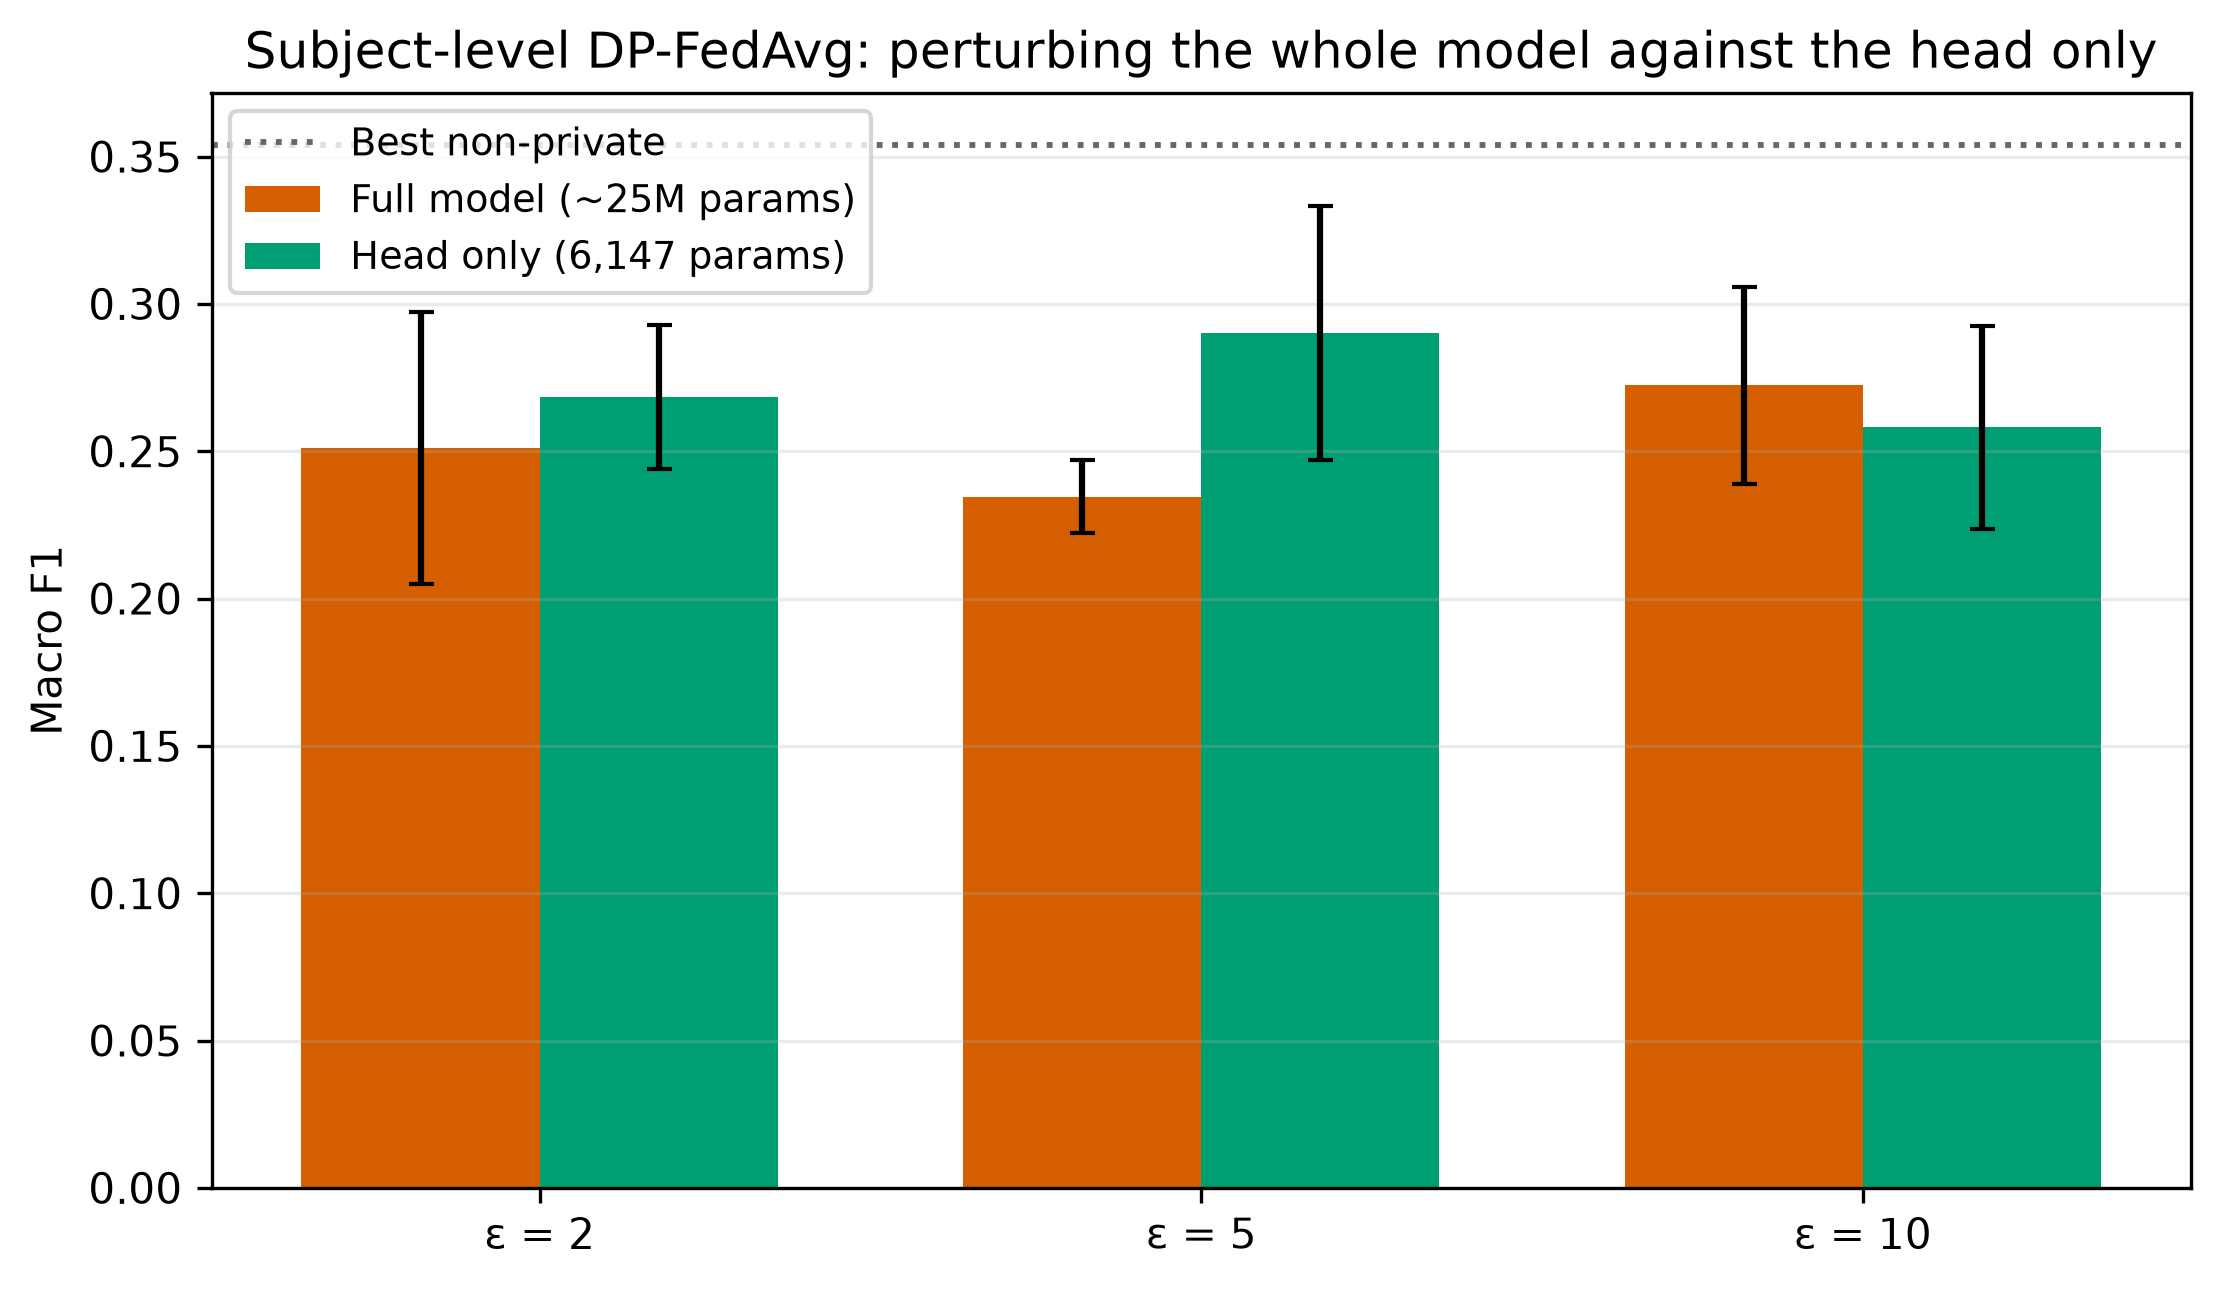
\includegraphics[width=\columnwidth]{dp_scope_comparison_v2.png}
  \caption{Subject-level DP-FedAvg macro F1 by perturbed dimension on
    the \SliceSubjects{}-subject slice cohort.  Restricting the Gaussian
    mechanism to the 6{,}147-parameter classifier head, rather than all
    $2.35\times10^{7}$ parameters, reduces the noise norm by roughly
    $62\times$ and recovers macro F1 at matched $\varepsilon$.  The
    dotted line is the best non-private result on that cohort; neither
    scope reaches it.}
  \label{fig:dp_scope}
\end{figure}

\subsection{Pixel-Space Explanation Similarity}

Table~\ref{tab:xai_similarity} reports Grad-CAM similarity between each
DP checkpoint and its matched non-DP reference on the slice cohort.
SSIM ranges only $0.20$--$0.34$ and Spearman rank correlation is
frequently at or below zero.  We report this for completeness and draw
no anatomical conclusion from it: these are heat maps over an
unregistered image grid, on models at near-chance accuracy, so a low
similarity is as consistent with both explanations being meaningless as
with one having moved.  The region-based analysis of
Section~\ref{sec:results-xai} is what replaced it, and the replacement
is the point --- a pixel-space explanation comparison on unregistered
volumes cannot be made to mean anything, however carefully it is
computed.

\begin{table}[t]
  \centering
  \caption{Grad-CAM similarity vs.\ matched non-DP reference, slice
  cohort, fold~0.  Reported for completeness; see the caution in the
  text.}
  \label{tab:xai_similarity}
  \renewcommand{\arraystretch}{1.15}
  \setlength{\tabcolsep}{2.5pt}
  \footnotesize
  \begin{tabular}{llccc}
    \toprule
    \textbf{Setting} & $\boldsymbol{\varepsilon}$ & \textbf{SSIM} & \textbf{Spearman} & \textbf{Dice@20\%} \\
    \midrule
    \multirow{3}{*}{Centralised, head-only DP}
      & 2  & 0.250 & 0.038  & 0.246 \\
      & 5  & 0.208 & $-$0.014 & 0.200 \\
      & 10 & 0.328 & 0.032  & 0.247 \\
    \multirow{3}{*}{Centralised, full-network DP}
      & 2  & 0.340 & 0.126  & 0.252 \\
      & 5  & 0.304 & 0.072  & 0.314 \\
      & 10 & 0.280 & 0.061  & 0.251 \\
    \multirow{3}{*}{FedAvg, head-only DP}
      & 2  & 0.244 & $-$0.026 & 0.200 \\
      & 5  & 0.269 & $-$0.038 & 0.201 \\
      & 10 & 0.245 & $-$0.005 & 0.207 \\
    FedAvg, full-network DP & 5 & 0.199 & $-$0.244 & 0.133 \\
    \bottomrule
  \end{tabular}
\end{table}

% ============================================================
\section{Privacy and Security Analysis}
\label{sec:privacy}
% ============================================================

\subsection{Threat Model}

\textit{Honest-but-Curious Server.}\;The server follows the FedAvg
protocol but attempts to infer information about individual clients from
received updates.  The subject-level Gaussian mechanism bounds the
influence of any one patient on the released model.

\textit{Gradient Inversion.}\;An adversary with access to shared updates
attempts to reconstruct training data~\cite{zhu2019}.  For the region
model the update is a 423-parameter delta over anatomical fractions;
per-subject clipping and additive noise bound what it reveals, and the
representation itself carries no voxel data to reconstruct.

\subsection{Formal Guarantees and Their Unit}

For the region model, the unit is the \emph{subject}: each participant's
total contribution is clipped to $C$ before noise, and the R\'enyi-DP
accountant composes across all rounds.  This is the guarantee stated in
Section~\ref{sec:problem} and it is the one a hospital needs.

For the \slicearm{} of Section~\ref{sec:legacy}, the sample-level runs
bound sensitivity at the \emph{slice} level: a subject contributing
several slices receives a looser effective per-subject guarantee than
the reported per-slice $\varepsilon$.  We state the unit explicitly
rather than let the two be conflated, and the discrepancy is one of the
reasons the subject-level mechanism was implemented.

$\delta = 10^{-3}$ throughout.  As noted in Section~\ref{sec:setup},
this is approximately $0.76/n$ at \CohSubjects{}~subjects and is looser
than convention now permits; it is a configuration choice inherited from
a much smaller cohort, not a requirement of the mechanism.

\subsection{Membership Inference on the Slice Pipeline}
\label{sec:mia_results}

Our original MIA evaluation used a loss-threshold attack whose decision
threshold was tuned on the very data being attacked, and re-derived
membership via a fresh random permutation that did not match the actual
training split.  Both defects invalidate the reported 88.9\% figure.  We
replaced it with two attacks whose ground truth is read directly from
each run's recorded train/test subject split and never re-derived: a
loss-threshold (Yeom) attack~\cite{yeom2018}, and a shadow-model attack
classifier~\cite{shokri2017} over (loss, confidence, entropy) features
pooled from 16~shadow ResNet50 models --- a documented simplification of
per-example LiRA~\cite{carlini2022}, which needs more shadow models per
example than this budget supports.  Both attacks score \emph{subjects},
aggregating per-slice scores before computing ROC.

Without DP, both centralised and federated ResNet50 are almost perfectly
vulnerable (AUC~0.994 and~0.961; 95.5\% and 72.7\% of true members
flagged at a 1\% false-positive rate), consistent with a model trained
on $\sim$22--26 subjects with augmentation.  Under every DP
configuration tested, MIA AUC collapses to near-chance (0.42--0.69),
essentially regardless of $\varepsilon$ within this noise floor.

\textbf{What this does and does not establish.}  It establishes that a
high-capacity network trained on a few dozen subjects memorises them,
and that DP-SGD removes that.  It does \emph{not} establish anything
about the system this paper proposes.  We have not run a membership
inference attack against the 423-parameter region model on
\CohSubjects{}~subjects, and its empirical vulnerability is therefore
unmeasured.  A model of that size on that many subjects has far less
capacity to memorise, so we would expect a weaker attack --- but
expecting is not measuring, and the formal subject-level guarantee is
the only privacy claim we make for the region model.  This is the
paper's largest outstanding gap and is the first experimental item in
Section~\ref{sec:future}.

\begin{table}[t]
  \centering
  \caption{Shadow-model MIA results (AUC / TPR@FPR=0.01) on the
  \slicearm{}, fold~0, seed~42.  No equivalent measurement exists for
  the region model; see the text.}
  \label{tab:mia}
  \renewcommand{\arraystretch}{1.15}
  \setlength{\tabcolsep}{3pt}
  \footnotesize
  \begin{tabular}{llcc}
    \toprule
    \textbf{Setting} & $\boldsymbol{\varepsilon}$ & \textbf{AUC} & \textbf{TPR@0.01} \\
    \midrule
    Centralised, no DP & $\infty$ & 0.994 & 0.955 \\
    FedAvg, no DP      & $\infty$ & 0.961 & 0.727 \\
    \midrule
    \multirow{3}{*}{Centralised, head-only DP}
      & 2  & 0.461 & 0.136 \\
      & 5  & 0.474 & 0.091 \\
      & 10 & 0.688 & 0.000 \\
    \multirow{3}{*}{Centralised, full-network DP}
      & 2  & 0.526 & 0.000 \\
      & 5  & 0.597 & 0.182 \\
      & 10 & 0.539 & 0.000 \\
    \multirow{3}{*}{FedAvg, head-only DP}
      & 2  & 0.442 & 0.000 \\
      & 5  & 0.565 & 0.000 \\
      & 10 & 0.416 & 0.000 \\
    FedAvg, full-network DP & 5 & 0.597 & 0.000 \\
    \bottomrule
  \end{tabular}
\end{table}

% ============================================================
\section{Verification and Reproducibility}
\label{sec:verification}
% ============================================================

The central claim of this paper is a negative one about evaluation
protocol, so the protocol itself has to be checkable rather than
asserted.  Three mechanisms do that.

\subsection{Automated Verification of the Split Property}

Subject-disjointness is asserted programmatically, not by inspection.  A
verification suite loads the shipped splits file and, for each fold,
checks that no subject appears in more than one of train, validation and
test, that no array index is reachable from two partitions, and that the
union of the three partitions is exactly the cohort.  The same suite
validates every recorded results file against a schema: required metrics
present, all metrics within $[0,1]$, and for every private run an
achieved $\varepsilon$ within 15\% of its target.  That last check
surfaced a real detail: the accountant's noise-multiplier search
overshoots the target budget by up to $0.2\%$, so the guarantee we
report is the \emph{achieved} $\varepsilon$ rather than the requested
one.

\subsection{Machine-Generated Tables}

Every numeric table is written into marker-delimited blocks in the
\LaTeX{} source by a generator that reads the aggregated results JSON
directly.  No result in a table is typed by hand, so a table cannot
drift from the experiment behind it.  A separate checker guards the
prose: it traces every percentage in the text to a recorded result and
fails on anything it cannot account for, with a small allow-list of
documented non-results such as chance rates and superseded figures.
That checker found a genuine defect during preparation: a sentence
citing an accuracy from one cohort beside a table holding another's.

\subsection{Test Suite and Continuous Integration}

The pure-logic modules --- splitting, client partitioning, model
construction, FedAvg and DP-FedAvg aggregation arithmetic, results
aggregation, statistical analysis --- are covered by a suite held at
100\% statement and branch coverage on that measured scope, enforced in
CI.  The CUDA training loops are excluded from measurement rather than
mocked: a mock of a training loop tests the mock.  Exclusions are
documented alongside the suite.  Tests run on synthetic fixtures and
need no ADNI access, so the pipeline is verifiable by a reader who
cannot obtain the data.

CI runs build, test, lint, package and demo deployment on every push, with
secret scanning and a coverage gate that fails the build.

\subsection{What Verification Did Not Catch}

Worth stating, since the paper argues for these mechanisms.  None of
them detected the orientation defect of
Section~\ref{sec:standardisation}.  The splits were valid, the schema
passed, coverage was complete, and every table matched its JSON.  The
defect lived in a single line that chose an array axis, produced no
error and no invalid value, and was consistent across runs.  Automated
verification protects against drift between a result and its report; it
does not protect against a pipeline that is measuring the wrong thing
consistently.  The only thing that caught this was inspecting the actual
extracted slices against anatomy, which no test suite was asking anyone
to do.

% ============================================================
\section{Limitations}
\label{sec:limitations}
% ============================================================

\textbf{No empirical privacy attack on the proposed model.}\;The
membership-inference results of Section~\ref{sec:mia_results} are
measured on the \slicearm{}.  The region model's empirical vulnerability
is unmeasured, so its privacy claim rests entirely on the formal
subject-level guarantee.  This is the paper's most significant gap.

\textbf{Clipping and noise are not separated.}\;The subject-level
mechanism clips per-subject deltas before adding noise.  We did not run
the clipping-only ($\sigma = 0$) control, so where private accuracy
meets or exceeds the non-private reference
(Section~\ref{sec:results-privacy}) we cannot attribute the effect to
the noise rather than to the clipping.

\textbf{Left--right handedness is measured for one series group and
inferred for four.}\;165 of the 272 degenerate-affine scans have their
mirror resolved by a determinant-consistency rule rather than by anchor
evidence (Section~\ref{sec:orientation}).  Harvard-Oxford features are
lateralised, so a wrong rule for a group would corrupt exactly the
features that matter.  The symmetrised-feature ablation that would
settle this is not run.

\textbf{Three seeds.}\;Every cell in
Tables~\ref{tab:v3-centralised}--\ref{tab:v3-privacy} is three seeds
(Section~\ref{sec:power}).  Differences of a few points with standard
deviations of one to three points are reported and not adjudicated.

\textbf{Privacy parameters inherited from a smaller cohort.}\;$\delta =
10^{-3}$ is approximately $0.76/n$ at \CohSubjects{}~subjects, and the
subject sampling rate $q \approx 0.8$ forgoes nearly all amplification
by subsampling.  Both were reasonable at 32~subjects and are loose now.

\textbf{The representation is a baseline, not a contribution.}\;Region
fractions over Harvard-Oxford with a linear classifier is a standard
morphometric approach, and \CohBinAcc{} on CN versus AD sits at the
lower end of what that literature
reports~\cite{cuingnet2011,kloppel2008}.  The paper's claims concern
measurement, privacy and explanation comparability, not diagnostic
performance.

\textbf{Simulated federation.}\;Clients are simulated over a real site
partition; network latency, heterogeneous hardware, asynchronous
training and client dropout are not modelled.

\textbf{Dataset scope.}\;ADNI represents a specific demographic and
geographic distribution.  Generalisation beyond it is untested, and the
male/female stratum difference observed in
Section~\ref{sec:results-confounds} is reported without explanation.

\textbf{No clinical claim.}\;Agreement with a reference model, or with
expected anatomy, is evidence about a model and not about a patient.
Nothing here should be read as evidence that these models are ready, or
close to ready, for clinical use.

% ============================================================
\section{Future Work}
\label{sec:future}
% ============================================================

The first four items require no new data and little compute, and we
regard them as prerequisites for the claims above rather than
extensions of them.

\textbf{Membership inference against the region model.}\;The shadow-model
attack of Section~\ref{sec:mia_results} applied to the 423-parameter
model on \CohSubjects{}~subjects, at every budget and non-private, so
that the empirical and formal privacy stories concern the same system.

\textbf{The clipping-only control.}\;$C = 1.0$ with $\sigma = 0$, to
separate regularisation by clipping from regularisation by noise in
Table~\ref{tab:v3-privacy}.

\textbf{Left--right-symmetrised ablation.}\;Averaging each region with
its contralateral partner makes the representation invariant to the
mirror, and re-running Table~\ref{tab:v3-centralised} on symmetrised
features would either retire the handedness limitation or expose it.

\textbf{More seeds, and tighter privacy parameters.}\;Ten seeds per cell
on a 423-parameter model, plus a sweep over $\delta$ and the subject
sampling rate $q$, would replace several of this paper's ``within the
spread'' statements with orderings.

\textbf{The balanced cohort.}\;Running the \CohortTotal{}-subject
specification of Section~\ref{sec:cohort-design}, on which a sex-only
rule is chance by construction.

\textbf{Adaptive budget allocation.}\;Per-round noise scheduling that
reduces $\sigma$ as convergence is detected, without increasing total
privacy cost.

\textbf{Personalised and multimodal federation.}\;Per-FedPer or
MAML-style personalisation against site heterogeneity, and joint
modelling of region features with clinical variables (MMSE, genetic
markers) following Pan et al.~\cite{pan2025}.

\textbf{Real deployment.}\;Asynchronous, dropout-tolerant aggregation on
distributed hospital infrastructure.

% ============================================================
\section{Conclusion}
\label{sec:conclusion}
% ============================================================

This paper is a corrected re-report of our own federated Alzheimer's
system, and its most transferable content is about measurement.

\textbf{Two defects, and the second was invisible.}\;Slice-level
splitting inflated accuracy from 19--36\% to 91--97\%.  Correcting it
left a near-chance residual we attributed to cohort size; the real cause
was that the pipeline chose its slice axis by array shape, extracting a
different anatomical plane depending on how each scanner wrote the file.
That defect raises no error, passes every schema check, and survives
complete test coverage.  A pipeline can be corrected into producing a
plausible number that is still measuring nothing.

\textbf{Standardisation makes the problem well posed.}\;With orientation
measured rather than assumed, every subject registered to MNI152, and
anatomy summarised as \CohFeatures{} named region fractions, a
423-parameter model reaches \CohTriAcc{} on three classes and
\CohBinAcc{} on CN versus AD subject-disjoint, and \CohTriSite{} and
\CohBinSite{} site-disjoint --- competent morphometric performance, and
the precondition for everything that follows.

\textbf{The usable regime of subject-level DP is set by dimension.}\;At
$d = 2.35\times10^{7}$ the mechanism collapses onto the majority class
while its accuracy rises; at $d = 423$ it stays usable to
$\varepsilon = 1$ at a cost of 3.5~points on CN versus AD.  The
dimension dependence is standard~\cite{bassily2014,tramer2021}; what we
add is its measurement across five orders of magnitude on one clinical
cohort, and the observation that the high-dimensional failure mode is
one an accuracy-only privacy--utility curve reports as a success.

\textbf{Explanations move faster than accuracy, and named regions make
that measurable.}\;Region attribution agreement with the non-private
reference falls from \CohXaiNonPrivate{} to \CohXaiTen{} at
$\varepsilon = 10$, where accuracy does not fall; the anatomy-anchored
medial-temporal share halves at $\varepsilon = 1$ where accuracy falls
3.5~points.  Wherever the explanation is part of the deliverable, an
accuracy-only privacy--utility curve understates the cost.

\textbf{What we have not shown.}\;The region model has not been attacked
empirically, clipping has not been separated from noise, and the
handedness of most degenerate-affine scans rests on a consistency rule.
Section~\ref{sec:future} lists these first because they are the claims a
reader should want before the rest.

% ============================================================
\section*{Acknowledgement}
% ============================================================

The authors thank Prof.\ Agha Alfi Mirza for project guidance and the
Department of Computer Science \& Engineering, PES University, Bangalore,
for institutional support.  Data collection and sharing were funded by the
Alzheimer's Disease Neuroimaging Initiative~(ADNI)
(NIH Grant U01~AG024904).  The investigators at ADNI contributed to the
design and implementation of ADNI and/or provided data, but did not
participate in the analysis or writing of this report.

% ============================================================
\balance
\begin{thebibliography}{25}

\bibitem{mitrovska2024}
A.~Mitrovska, P.~Safari, K.~Ritter, B.~Shariati, and J.~K.~Fischer,
``Secure federated learning for Alzheimer's disease detection,''
\textit{Front.\ Aging Neurosci.}, vol.~16, p.~1324032, Mar.~2024.

\bibitem{mastoi2025}
Q.~Mastoi, S.~Latif, S.~Brohi, J.~Ahmad, A.~Alqhatani,
M.~S.~Alshehri, A.~Al~Mazroa, and R.~Ullah,
``Explainable AI in medical imaging: An interpretable and collaborative
federated learning model for brain tumor classification,''
\textit{Front.\ Oncol.}, vol.~15, p.~1535478, Jan.~2025.

\bibitem{pan2025}
J.~Pan, Z.~Fan, G.~E.~Smith, Y.~Guo, J.~Bian, and J.~Xu,
``Federated learning with multi-cohort real-world data for predicting
the progression from mild cognitive impairment to Alzheimer's disease,''
\textit{Alzheimer's Dement.}, vol.~21, no.~4, p.~e70128, 2025.

\bibitem{privacy2024}
G.~Kaissis, M.~Makowski, D.~R\"{u}ckert, and R.~Braren,
``Privacy-preserving federated learning and uncertainty quantification
in medical imaging,''
\textit{Radiol.\ Artif.\ Intell.}, p.~240637, 2024.

\bibitem{evolutionary2025}
N.~Basnin, T.~Mahmud, R.~U.~Islam, and K.~Andersson,
``An evolutionary federated learning approach to diagnose Alzheimer's
disease under uncertainty,''
\textit{Diagnostics}, vol.~15, no.~1, p.~80, 2025.

\bibitem{mcmahan2017}
H.~B.~McMahan, E.~Moore, D.~Ramage, S.~Hampson, and B.~A.~y~Arcas,
``Communication-efficient learning of deep networks from decentralized
data,''
in \textit{Proc.\ 20th Int.\ Conf.\ Artif.\ Intell.\ Statist.\
(AISTATS)}, 2017, pp.~1273--1282.

\bibitem{bonawitz2017}
K.~Bonawitz et al.,
``Practical secure aggregation for privacy-preserving machine learning,''
in \textit{Proc.\ ACM SIGSAC Conf.\ Comput.\ Commun.\ Secur.\ (CCS)},
2017, pp.~1175--1191.

\bibitem{dwork2014}
C.~Dwork and A.~Roth,
``The algorithmic foundations of differential privacy,''
\textit{Found.\ Trends Theor.\ Comput.\ Sci.}, vol.~9, no.~3--4,
pp.~211--407, 2014.

\bibitem{abadi2016}
M.~Abadi et al.,
``Deep learning with differential privacy,''
in \textit{Proc.\ ACM SIGSAC Conf.\ Comput.\ Commun.\ Secur.\ (CCS)},
2016, pp.~308--318.

\bibitem{gradcam}
R.~R.~Selvaraju, M.~Cogswell, A.~Das, R.~Vedantam, D.~Parikh, and
D.~Batra,
``Grad-CAM: Visual explanations from deep networks via gradient-based
localization,''
in \textit{Proc.\ IEEE Int.\ Conf.\ Comput.\ Vis.\ (ICCV)}, 2017,
pp.~618--626.

\bibitem{shap}
S.~M.~Lundberg and S.-I.~Lee,
``A unified approach to interpreting model predictions,''
in \textit{Adv.\ Neural Inf.\ Process.\ Syst.\ (NeurIPS)}, 2017,
pp.~4765--4774.

\bibitem{vgg19}
K.~Simonyan and A.~Zisserman,
``Very deep convolutional networks for large-scale image recognition,''
in \textit{Proc.\ Int.\ Conf.\ Learn.\ Represent.\ (ICLR)}, 2015.

\bibitem{resnet50}
K.~He, X.~Zhang, S.~Ren, and J.~Sun,
``Deep residual learning for image recognition,''
in \textit{Proc.\ IEEE Conf.\ Comput.\ Vis.\ Pattern Recognit.\
(CVPR)}, 2016, pp.~770--778.

\bibitem{opacus}
A.~Yousefpour et al.,
``Opacus: User-friendly differential privacy library in PyTorch,''
\textit{arXiv preprint arXiv:2109.12298}, 2021.

\bibitem{adni}
R.~C.~Petersen et al.,
``Alzheimer's Disease Neuroimaging Initiative (ADNI): Clinical
characterization,''
\textit{Neurology}, vol.~74, no.~3, pp.~201--209, Jan.~2010.

\bibitem{zhu2019}
L.~Zhu, Z.~Liu, and S.~Han,
``Deep leakage from gradients,''
in \textit{Adv.\ Neural Inf.\ Process.\ Syst.\ (NeurIPS)}, 2019,
pp.~14747--14756.

\bibitem{shokri2017}
R.~Shokri, M.~Stronati, C.~Song, and V.~Shmatikov,
``Membership inference attacks against machine learning models,''
in \textit{Proc.\ IEEE Symp.\ Secur.\ Priv.\ (SP)}, 2017, pp.~3--18.

\bibitem{yeom2018}
S.~Yeom, I.~Giacomelli, M.~Fredrikson, and S.~Jha,
``Privacy risk in machine learning: Analyzing the connection to
overfitting,''
in \textit{Proc.\ IEEE 31st Comput.\ Secur.\ Found.\ Symp.\ (CSF)},
2018, pp.~268--282.

\bibitem{carlini2022}
N.~Carlini, S.~Chien, M.~Nasr, S.~Song, A.~Terzis, and F.~Tram\`{e}r,
``Membership inference attacks from first principles,''
in \textit{Proc.\ IEEE Symp.\ Secur.\ Priv.\ (SP)}, 2022, pp.~1897--1914.

\bibitem{tramer2021}
F.~Tram\`{e}r and D.~Boneh,
``Differentially private learning needs better features (or much more
data),''
in \textit{Proc.\ Int.\ Conf.\ Learn.\ Represent.\ (ICLR)}, 2021.

\bibitem{bassily2014}
R.~Bassily, A.~Smith, and A.~Thakurta,
``Private empirical risk minimization: Efficient algorithms and tight
error bounds,''
in \textit{Proc.\ IEEE 55th Annu.\ Symp.\ Found.\ Comput.\ Sci.\
(FOCS)}, 2014, pp.~464--473.

\bibitem{yu2021}
D.~Yu, H.~Zhang, W.~Chen, and T.-Y.~Liu,
``Do not let privacy overbill utility: Gradient embedding perturbation
for private learning,''
in \textit{Proc.\ Int.\ Conf.\ Learn.\ Represent.\ (ICLR)}, 2021.

\bibitem{mcmahan2018}
H.~B.~McMahan, D.~Ramage, K.~Talwar, and L.~Zhang,
``Learning differentially private recurrent language models,''
in \textit{Proc.\ Int.\ Conf.\ Learn.\ Represent.\ (ICLR)}, 2018.

\bibitem{kairouz2021}
P.~Kairouz et al.,
``Advances and open problems in federated learning,''
\textit{Found.\ Trends Mach.\ Learn.}, vol.~14, no.~1--2, pp.~1--210,
2021.

\bibitem{cuingnet2011}
R.~Cuingnet, E.~Gerardin, J.~Tessieras, G.~Auzias, S.~Leh\'{e}ricy,
M.-O.~Habert, M.~Chupin, H.~Benali, and O.~Colliot,
``Automatic classification of patients with Alzheimer's disease from
structural MRI: A comparison of ten methods using the ADNI database,''
\textit{NeuroImage}, vol.~56, no.~2, pp.~766--781, 2011.

\bibitem{kloppel2008}
S.~Kl\"{o}ppel, C.~M.~Stonnington, C.~Chu, B.~Draganski,
R.~I.~Scahill, J.~D.~Rohrer, N.~C.~Fox, C.~R.~Jack,
J.~Ashburner, and R.~S.~J.~Frackowiak,
``Automatic classification of MR scans in Alzheimer's disease,''
\textit{Brain}, vol.~131, no.~3, pp.~681--689, 2008.

\end{thebibliography}

\end{document}
